 % The main file for CAMP reports
 % Don't put any content in here.
 % Don't even include content files by using \input or \inlcude.
 % Put your content to TEXT.TEX or include it there using \input.
 % Uses:
 %		SETTINGS.TEX	contains the settings for this document
 %		COMMANDS.TEX	contains commands which can be used while writing
 %		INFO.TEX			contains the author, title and so on for the cover
 %		COVER.TEX			formats the front cover of the document
 %		ABSTRACT.TEX	contains the abstract to be included (if needed)
 %		TEXT.TEX			contains the actual content of the document
 %		BIB.BIB				containt the BibTeX entries for the document


%% Draft document mode
%% Final document
\documentclass[11pt,a4paper,bibtotoc,idxtotoc,headsepline,footsepline,footexclude,BCOR14mm,DIV13]{scrbook}

%\documentclass[11pt,a4paper,bibtotoc,idxtotoc,headsepline,footsepline,footexclude,BCOR20mm,DIV10]{scrbook}

% KOMA-Optionen:
%  bibtotoc: include bibliography in table of contents
%  idxtotoc: include index in table of contents
%  headsepline: use horizontalline under heading
%  BCOR: binding correcion (Bindungskorrektur) (e.g.: BCOR5mm)
%  DIV: Number of sheet sections (used for layout) (e.g.: DIV12)



% include title and author information for the cover
% Set here the title, authors and other stuff to be used for the cover
% This file is used by MAIN.TEX

% set title, authors and stuff for the cover
\def\doctype{Bachelor's Thesis in Informatics}
\def\title{Reinforcement Learning for Path Planing of Robotic Arms}
\def\titleGer{Bestärkendes Lernen zur Pfadplanung von robotischen Armen}
\def\author{Anton Mai}
\def\date{February 17, 2020}

% text to appear in the footer
\def\footertext{}


% include settings
\PassOptionsToPackage{table,svgnames,dvipsnames}{xcolor}

\usepackage[utf8]{inputenc}
\usepackage[T1]{fontenc}
\usepackage[sc]{mathpazo}
\usepackage[ngerman,american]{babel}
\usepackage[autostyle]{csquotes}
\usepackage[%
  backend=biber,
  url=false,
  style=alphabetic,
  maxnames=4,
  minnames=3,
  maxbibnames=99,
  giveninits,
  uniquename=init]{biblatex} % TODO: adapt citation style
\usepackage{graphicx}
\usepackage{scrhack} % necessary for listings package
\usepackage{listings}
\usepackage{lstautogobble}
\usepackage{tikz}
\usepackage{pgfplots}
\usepackage{pgfplotstable}
\usepackage{booktabs}
\usepackage[final]{microtype}
\usepackage{caption}
\usepackage[hidelinks]{hyperref} % hidelinks removes colored boxes around references and links

\bibliography{bibliography}

\setkomafont{disposition}{\normalfont\bfseries} % use serif font for headings
\linespread{1.05} % adjust line spread for mathpazo font

% Add table of contents to PDF bookmarks
\BeforeTOCHead[toc]{{\cleardoublepage\pdfbookmark[0]{\contentsname}{toc}}}

% Define TUM corporate design colors
% Taken from http://portal.mytum.de/corporatedesign/index_print/vorlagen/index_farben
\definecolor{TUMBlue}{HTML}{0065BD}
\definecolor{TUMSecondaryBlue}{HTML}{005293}
\definecolor{TUMSecondaryBlue2}{HTML}{003359}
\definecolor{TUMBlack}{HTML}{000000}
\definecolor{TUMWhite}{HTML}{FFFFFF}
\definecolor{TUMDarkGray}{HTML}{333333}
\definecolor{TUMGray}{HTML}{808080}
\definecolor{TUMLightGray}{HTML}{CCCCC6}
\definecolor{TUMAccentGray}{HTML}{DAD7CB}
\definecolor{TUMAccentOrange}{HTML}{E37222}
\definecolor{TUMAccentGreen}{HTML}{A2AD00}
\definecolor{TUMAccentLightBlue}{HTML}{98C6EA}
\definecolor{TUMAccentBlue}{HTML}{64A0C8}

% Settings for pgfplots
\pgfplotsset{compat=newest}
\pgfplotsset{
  % For available color names, see http://www.latextemplates.com/svgnames-colors
  cycle list={TUMBlue\\TUMAccentOrange\\TUMAccentGreen\\TUMSecondaryBlue2\\TUMDarkGray\\},
}

% Settings for lstlistings
\lstset{%
  basicstyle=\ttfamily,
  columns=fullflexible,
  autogobble,
  keywordstyle=\bfseries\color{TUMBlue},
  stringstyle=\color{TUMAccentGreen}
}


% include commands
% Commands to be used within the TUM report document
% Included by MAIN.TEX
% Please include your own cool commands here. 
% Be only sure to comment it sufficiently so others can use it.

%-------------------------------------------------------------
%                      Own Commands
%-------------------------------------------------------------


%-------------------------------------------------------------
% math stuff -------------------------------------------------

% nice R, N, C
\newcommand{\nat}{\mathbb{N}}
\newcommand{\real}{\mathbb{R}}
\newcommand{\compl}{\mathbb{C}}



% norm
\newcommand{\norm}[1]{\left\| #1 \right\|}

% un demi
\newcommand{\half}{\frac{1}{2}}

% parantheses
\newcommand{\parenth}[1]{ \left( #1 \right) }
\newcommand{\bracket}[1]{ \left[ #1 \right] }
\newcommand{\accolade}[1]{ \left\{ #1 \right\} }
%\newcommand{\angle}[1]{ \left\langle  #1 \right\rangle }

% partial derivative: %#1 function, #2 which variable
% simple / single line version
\newcommand{\pardevS}[2]{ \delta_{#1} f(#2) }
% fraction version
\newcommand{\pardevF}[2]{ \frac{\partial #1}{\partial #2} }

% render vectors: 3 and 4 dimensional
\newcommand{\veciii}[3]{\left[ \begin{array}[h]{c} #1 \\ #2 \\ #3	\end{array} \right]}
\newcommand{\veciv}[4]{\left[ \begin{array}[h]{c} #1 \\ #2 \\ #3 \\ #4	\end{array} \right]}

% render matrices: 3  dimensional (arguments in row first order)
\newcommand{\matiii}[9]{\left[ \begin{array}[h]{ccc} #1 & #2 & #3 \\ #4 & #5 & #6 \\ #7 & #8 & #9	\end{array} \right]}
%DOESN'T WORK,DON'T KNOW WHY \newcommand{\mativ}[16]{\left[ \begin{array}[h]{cccc} #1 & #2 & #3 & #4 \\ #5 & #6 & #7 & #8 \\ #9 & #10 & #11 & #12 \\ #13 & #14 & #15 & #16 \end{array} \right]}


%-------------------------------------------------------------
%-------------------------------------------------------------


%-------------------------------------------------------------
% some abreviations ------------------------------------------
\newcommand{\Reg}{$^{\textregistered}$}
\newcommand{\reg}{$^{\textregistered}$ }
\newcommand{\Tm}{\texttrademark}
\newcommand{\tm}{\texttrademark~}
\newcommand {\bsl} {$\backslash$}

%-------------------------------------------------------------
%-------------------------------------------------------------


%-------------------------------------------------------------
% formating --------------------------------------------------

% Theorem & Co environments and counters
\newtheorem{theorem}{Theorem}[chapter]
\newtheorem{lemma}[theorem]{Lemma}
\newtheorem{corollary}[theorem]{Corollary}
\newtheorem{remark}[theorem]{Remark}
\newtheorem{definition}[theorem]{Definition}
\newtheorem{equat}[theorem]{Equation}
\newtheorem{example}[theorem]{Example}
\newtheorem{algorithm}[theorem]{Algorithm}

% inserting figures
\newcommand{\insertfigure}[4]{ % Filename, Caption, Label, Width percent of textwidth
	\begin{figure}[htbp]
		\begin{center}
			\includegraphics[width=#4\textwidth]{#1}
		\end{center}
		\vspace{-0.4cm}
		\caption{#2}
		\label{#3}
	\end{figure}
}




% referecing figures

\newcommand{\refFigure}[1]{ %label
	figure \ref{#1}
}
\newcommand{\refChapter}[1]{ %label
	chapter \ref{#1}
}

\newcommand{\refSection}[1]{ %label
	section \ref{#1}
}

\newcommand{\refParagraph}[1]{ %label
	paragraph \ref{#1}
}

\newcommand{\refEquation}[1]{ %label
	equation \ref{#1}
}

\newcommand{\refTable}[1]{ %label
	table \ref{#1}
}




\newcommand{\rigidTransform}[2]
{
	${}^{#2}\!\mathbf{H}_{#1}$
}

%code, in typewriter
\newcommand{\code}[1]
 {\texttt{#1}}

% comment that appears on the border - very practical !!!
\newcommand{\comment}[1]{\marginpar{\raggedright \noindent \footnotesize {\sl #1} }}

% page clearing
\newcommand{\clearemptydoublepage}{%
  \ifthenelse{\boolean{@twoside}}{\newpage{\pagestyle{empty}\cleardoublepage}}%
  {\clearpage}}


%-------------------------------------------------------------
%-------------------------------------------------------------


\newcommand{\etAl}{\emph{et al.}\mbox{ }}

\pdfinfo{
   /Author (Anton Mai)
   /Title (Reinforcement Learning for Path Planing of Robotic Arms)
   /Keywords (RL, Path Planning, Robotic Arms, HER)
}

\hypersetup{%
pdftitle={Reinforcement Learning for Path Planing of Robotic Arms},%
pdfauthor={Anton Mai},%
pdfkeywords={RL, Path Planning, Robotic Arms, HER},%
}%

\hypersetup{
    colorlinks=false,
    pdfborder={0 0 0},
}


%\makeindex
	%% inter line spacing
%\linespread{1.0}

\makeglossary

\begin{document}

	\frontmatter
	
	
	\begin{titlepage}
  % HACK for two-sided documents: ignore binding correction for cover page.
  % Adapted from Markus Kohm's KOMA-Script titlepage=firstiscover handling.
  % See http://mirrors.ctan.org/macros/latex/contrib/koma-script/scrkernel-title.dtx,
  % \maketitle macro.
  \oddsidemargin=\evensidemargin\relax
  \textwidth=\dimexpr\paperwidth-2\evensidemargin-2in\relax
  \hsize=\textwidth\relax

  \centering

  \IfFileExists{logos/tum.pdf}{%
    \includegraphics[height=20mm]{logos/tum.pdf}
  }{%
    \vspace*{20mm}
  }

  \vspace{5mm}
  {\huge\MakeUppercase{\getFaculty{}}}\\

  \vspace{5mm}
  {\large\MakeUppercase{\getUniversity{}}}\\

  \vspace{20mm}
  {\Large \getDoctype{}}

  \vspace{15mm}
  {\huge\bfseries \getTitle{}}

  \vspace{15mm}
  {\LARGE \getAuthor{}}

  \IfFileExists{logos/faculty.pdf}{%
    \vfill{}
    \includegraphics[height=20mm]{logos/faculty.pdf}
  }{}
\end{titlepage}

%	\clearemptydoublepage
%	
%	% The titlepage for the CAMP report document.
% Included by MAIN.TEX


%--------------------------------------------------
% The title page
%--------------------------------------------------

% correct BCOR - undo at the end !!!
\def\bcorcor{0.15cm}
\addtolength{\hoffset}{\bcorcor}

\thispagestyle{empty}

 \vspace{10mm}
\begin{center}
	       \oTUM{4cm}
	   
	   \vspace{5mm}     
	   %\huge FAKULT{\"A}T F{\"U}R INFORMATIK\\ 
	   \huge DEPARTMENT OF INFORMATICS \\
	   \vspace{0.5cm}
	 %\large DER TECHNISCHEN UNIVERSIT{\"A}T M{\"U}NCHEN\\
	 \large TECHNISCHE UNIVERSIT{\"A}T M{\"U}NCHEN\\
        
	\end{center}
		

\vspace{10mm}
\begin{center}

   {\Large \doctype}

  \vspace{10mm}
  
  {\LARGE \title}\\
  
  
  \vspace{10mm}
  
  
  {\LARGE  \titleGer}\\
  
  
  \vspace{10mm}

    %\hfill
    \begin{tabular}{ll}
	   \Large Author:     & \Large \author \\[2mm]
	   \Large Supervisor:    & \Large Prof. Dr.-Ing. habil. Alois Knoll \\[2mm]
	   \Large Advisors:	& \Large Dr. Kai Huang\\ 
	                    & \Large Biao Hu, M.Sc.\\[2mm]
	   \Large Date:       & \Large April 15, 2015
	 \end{tabular}
	 
	 \vspace{5mm}
	 
	 \begin{figure}[h!]
  \centering
   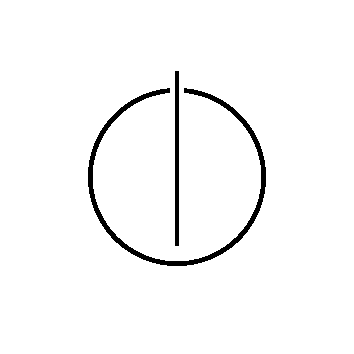
\includegraphics[width=4cm]{styles/informat.png}
  \end{figure}
   

\end{center}

% undo BCOR correction
\addtolength{\hoffset}{\bcorcor}

	
	
%	\input{components/cover_maschmeyer}
	\clearemptydoublepage
	
	% The titlepage for the CAMP report document.
% Included by MAIN.TEX


%--------------------------------------------------
% The title page
%--------------------------------------------------

% correct BCOR - undo at the end !!!
\def\bcorcor{0.15cm}
\addtolength{\hoffset}{\bcorcor}

\thispagestyle{empty}

 \vspace{10mm}
\begin{center}
	       \oTUM{4cm}
	   
	   \vspace{5mm}     
	   %\huge FAKULT{\"A}T F{\"U}R INFORMATIK\\ 
	   \huge DEPARTMENT OF INFORMATICS \\
	   \vspace{0.5cm}
	 %\large DER TECHNISCHEN UNIVERSIT{\"A}T M{\"U}NCHEN\\
	 \large TECHNISCHE UNIVERSIT{\"A}T M{\"U}NCHEN\\
        
	\end{center}
		

\vspace{10mm}
\begin{center}

   {\Large \doctype}

  \vspace{10mm}
  
  {\LARGE \title}\\
  
  
  \vspace{10mm}
  
  
  {\LARGE  \titleGer}\\
  
  
  \vspace{10mm}

    %\hfill
    \begin{tabular}{ll}
	   \Large Author:     & \Large \author \\[2mm]
	   \Large Supervisor:    & \Large Prof. Dr.-Ing. habil. Alois Knoll \\[2mm]
	   \Large Advisors:	& \Large Dr. Kai Huang\\ 
	                    & \Large Biao Hu, M.Sc.\\[2mm]
	   \Large Date:       & \Large April 15, 2015
	 \end{tabular}
	 
	 \vspace{5mm}
	 
	 \begin{figure}[h!]
  \centering
   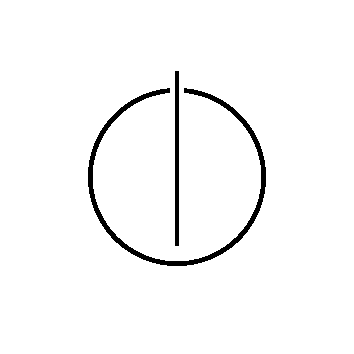
\includegraphics[width=4cm]{styles/informat.png}
  \end{figure}
   

\end{center}

% undo BCOR correction
\addtolength{\hoffset}{\bcorcor}

	
	
	\clearemptydoublepage


\thispagestyle{empty}
\selectlanguage{german}
	\vspace*{0.8\textheight}
	\noindent
	%Ich versichere, dass ich diese Diplomarbeit selbst{\"a}ndig verfasst und nur 
	%die angegebenen \\Quellen und Hilfsmittel verwendet habe.
	
	I confirm that this bachelor's thesis is my own work and I have documented all sources and material used.
	
	%TODO check space
	\vspace{15mm}
	\noindent
	M{\"u}nchen, \today \hspace{5cm} \author
\selectlanguage{english}
\newpage

	
	%\clearemptydoublepage
\phantomsection
\addcontentsline{toc}{chapter}{Acknowledgements}	


%\chapter*{Acknowledgements}

\vspace*{2cm}

\begin{center}
{\Large \bf Acknowledgments}
\end{center}

\vspace{1cm}




If someone contributed to the thesis... might be good to thank them here.
	
	% Abstract for the TUM report document
% Included by MAIN.TEX


\clearemptydoublepage
\phantomsection
\addcontentsline{toc}{chapter}{Abstract}





\vspace*{2cm}
\begin{center}
{\Large \bf Abstract}
\end{center}
\vspace{1cm}

%An abstracts abstracts the thesis!

Heterogeneous computing systems consisting of CPUs, GPUs and FPGAs currently suffer from a comparatively low bandwidth and high latency for data transfers between the GPU and the FPGA.
So far, no standard or vendor-provided method exists for direct communication between these two devices.
Indirect communication with a round-trip via the CPU is required.

This thesis enables this missing link over the PCIe bus for use with the popular high performance computing platform OpenCL.
%opencl
As expected, a significant increase in bandwidth has been achieved.
However, only the direction from the FPGA to the GPU could be realized.
More investigation or a different approach is still required to enable the opposite direction as well.





	\tableofcontents

%  \clearemptydoublepage

\phantomsection
\addcontentsline{toc}{chapter}{Outline of the Thesis}

\begin{center}
	\huge{Outline of the Thesis}
\end{center}




%--------------------------------------------------------------------
\section*{Part I: Introduction and Theory}

\noindent {\scshape Chapter 1: Introduction}  \vspace{1mm}

\noindent  This chapter presents an overview of the thesis and it purpose. Furthermore, it will discuss the sense of life in a very general approach.  \\

\noindent {\scshape Chapter 2: Theory}  \vspace{1mm}

\noindent  No thesis without theory.   \\

%--------------------------------------------------------------------
\section*{Part II: The Real Work}

\noindent {\scshape Chapter 3: Overview}  \vspace{1mm}

\noindent  This chapter presents the requirements for the process.
   \clearemptydoublepage

\phantomsection
\addcontentsline{toc}{chapter}{List of Abbreviations}

\begin{center}
	\huge{List of Abbreviations}
\end{center}


\vspace{3cm}


\begin{center}
\begin{tabular}{l p{12cm}}
	ATT & Address Translation Table in the Altera PCIe core\\
	BAR & PCI Base Address Register\\
	BSP & Board Support Package, IP stack for Altera OpenCL\\
	CPU & Central Processing Unit\\
	DDR & Double Data Rate, a type of memory\\
	DMA & Direct Memory Access\\
	DPU & Double-precision Floating Point Unit\\
	FIFO & First-In First-Out Queue\\
	FPGA & Field Programmable Gate Array\\
	GPGPU & General Purpose Computing on Graphics Processing Units\\
	GPU & Graphics Processing Unit\\
	HDL & Hardware Description Language\\
	HPC & High Performance Computing\\
	ICD & Installable Client Driver, library that acts as a proxy between different OpenCL implementations\\
	IOMMU & Input/Output Memory Management Unit\\
	IP  & Intellectual Property, usually refers to HDL code\\
	IPC & Inter-Process Communication\\
	LUT & Look-Up Table, refers to the basic FPGA building block\\
	MMIO & Memory Mapped Input/Output\\
	MMU & Memory Management Unit\\
	OpenCL & Open Computing Language, a popular HPC platform\\
	OS  & Operating System\\
	PCIe & Peripheral Component Interconnect Express Bus\\
	RAM & Random Access Memory\\
	RDMA & Remote Direct Memory Access\\
	SDK & Software Development Kit\\
	SMX & NVIDIA Streaming Multiprocessor\\
	
\end{tabular}
\end{center}


	\mainmatter
	
	
		% ---------------------------------------------------------------------------
		%
		%Introduction and Background Theory
		%
		% ---------------------------------------------------------------------------
		%\part[Introduction and Theory]{Introduction and Theory}
		%\label{part:introAndBackgroundTheory}
		\chapter{Introduction}


%%recent advances in machine learning
%% alphago, more examples. 
%TODO use alphago zero, it is stronger

Lee Sedol, one of the best Go players in the world, was beaten by the Go engine AlphaGo in a match. The engine was clearly stronger \cite{leesedol}.  
%TODO /cite{leesedol}
AlphaGo only knew the rules at the beginning and got stronger only by playing with itself. 
Artificial Intelligence is quite popular nowadays because of its many use cases: Self-Driving cars, playing atari games, robotics and more. 
But how do these engines learn how to get so good at their areas ? The answer is reinforcement learning, an area of machine learning. 

\vspace{0.5cm}

The idea of reinforcement learning is to have a state and actions that an agent can choose from. Each action results in different rewards and states. Rewards are used by agent to measure how good an action was. This process is repeated which results in the agent learning which actions in each state are better.
%TODO maybe find a better example with better reward
Imagine you are a soccer player. You are standing in front of the goal (which is the state you are in). You can either shoot or pass the ball (which are your available actions). You choose to shoot, but the ball is blocked by the goalkeeper (you got a low reward). So the next time you are in front of the goal again, you will more probably try to pass the ball. This time your teammate scored a goal (you got a high reward). From this experience you learn that it is probably better to pass the ball if you are standing in front of the goal.
The concept of reinforcement learning can be used in a variety of environments, for example robotic arms.

\vspace{0.5cm}

%%robotic arms uses

Already in the 14th century, Leonardo da Vinci made blueprints of robotic arms.
%TODO \cite{roboarmhistory} 

A robotic arm resembles a human arm. It consists of segments which are connected by joints. 
%TODO \cite{howroboarmworks}
The number of joints correspond to what is called Degrees of Freedom. A robotic arm with 5 joints would have 5 Degrees of Freedom because it can pivot in 5 ways. Each joint is connected to a step motor. Step motors make the robot move very precisely.
The equivalent to a human hand is the end effector. The end effector can vary depending on the tasks.  

\vspace{0.5cm}

Robotic arms have many advantages. They are very accurate and consistent which is why they are mostly used for repetitive tasks or tasks that require high accuracy which are hard for humans. 
%TODO \cite{roboarmuk} 
This is the main reason why they are used in laboratories and hospitals for surgeries. They can also be used automatically without any human which is why they are used for manufacturing and assembly lines. 

\vspace{0.5cm}

Humans still have to teach the robotic arms how to move when 
setting them up. For path planning of the robotic arm, a sequence of actions has to be found that solves the task. This sequence is saved and repetitively executed by the robotic arm. Finding the path still requires human labor. Either by testing or by using linear algebra a path can be found. 
%TODO find good cite 
A robotic arm needs 6 Degrees of Freedom to be able to move its end effector in every direction and orientation. This also means that robotic arms with more degrees of freedom do not have a unique path to solve the tasks. There are different paths which can vary in length and energy consumption.
To improve the quality of the path and to do path planning without a human, using reinforcement learning for robotic arms is a logical approach. 

\vspace{0.5cm}


%%reinforcement learning in robotics
%TODO cite papers with rl robotics
...

\vspace{0.5cm}

%%problems with reinforcement learning because of sparse rewards

There is an issue that prevents robotic arms to learn with reinforcement learning. It is hard to construct a suitable reward function for tasks where robotic arms are used. For example ... 
%TODO read HER paper, cite
So either a suitable reward function has to be constructed by hand, or the simplest reward function, a binary sparse reward function has to be used. 
Both approaches have some issues. 
Constructing a reward function can be quite complicated. Also, for each task an individual reward function has to be made. So someone has to do this work which defeats the purpose of using reinforcement learning for robotic arms over path planning by hand. Depending on the case it might be easier to just plan the path without reinforcement learning.
Using only a sparse reward for robotic arms is as follows. a reward is given, when the goal is reached, no reward is given when the goal is not reached. Robotic arms have usually many Degrees of Freedom, so there are many actions that can be taken by the robotic arm. It is quite unlikely for robotic arms to fulfill the task by doing random movements. Tasks like moving an object are near impossible to solve with random actions. 
%TODO Find prove-> at timestep 0 for fetchplace 
So it is very unlikely for the robotic arm to earn a reward and learn. It takes a very long time to train a robotic arm with sparse rewards.
But recently hindsight experience replay has been introduced. 
%TODO \cite HERPAPER]
Hindsight experience replay allows a high learning rate even with sparse rewards. 


\vspace{0.5cm}

%%her introduces

Hindsight experience replay works as follows.


\vspace{0.5cm}

%%many endeavors to use and improve her


%% some robotic arm tasks , eg. stacking stones
%%mostly work on improving her

\vspace{0.5cm}

%%using harder environments for her in this thesis to see if it also works.



This thesis is structured as follows: 
Chapter 2 describes the theoretical background on robotic arms, reinforcement learning and algorithms like deep deterministic policy gradients and hindsight experience replay. 
Chapter 3 explains the methodology used for this thesis.
Chapter 4 gives an overview of the simulation environment.
In chapter 5, the experiments are presented and the results are discussed.
In the last chapter, the results are summarized and suggestions for further work is provided.





		
		\chapter{Theoretical Background}

This chapter explains the concepts needed to understand this thesis. The theory behind RL, ANN, DDPG and HER is explained.

\section{Reinforcement Learning}
%% In context of machine learning (supervised,unsupervised)
%% potential to be better than humans

RL is one of the main learning concepts of Machine Learning next to Supervised Learning and Unsupervised Learning \cite{machinelearning}.
\newline
In Supervised Learning some input data is given to the learning agent. The agent is expected to come up with some output which is then compared with the expected output. If the output given by the agent and the expected output matches, then the agent was correct. The agent is trained by calculating the error between expected output and actual output. An use case for Supervised Learning is sorting mails into regular mail and spam mail. The agent is given a mail and it should decide whether the mail is regular or spam based on the content. Supervised Learning is used for classification and regression problems \cite{machinelearning}. It is mainly useful when the expected output is already known, so the learning agent can learn to do recognize these. 
\newline
In Unsupervised Learning there is no expected output. The learning agent is fed with data so it can figure out interesting features and similarities between different data. Unsupervised Learning is often used to cluster data, often pictures, based on similarities \cite{machinelearning}.
\newline
In RL the agent is learning through rewards that are given through interaction with an environment. The goal of a task is clear, but the path of actions to reach the goal is not trivial. RL is used to find the best action in each situation. It is often used for games because they are already set up to have a clear task and goal, but the optimal way to reach it is not clear. Games usually provide full information on the environment in contrast to the real world, therefore setting up the learning environment is simple. Also Supervised Learning is limited in performance because the agent can only learn to become as good the expected output that we set. So in games like chess, with Supervised Learning the agent can only become as good as the best players it learns from, but not better. It is limited by the skills of the best humans \cite{nolimit}. However, RL is not restricted by these limitations. The agent can improve on its own only by exploring his options. In games like Go and Chess, engines that use RL have already far surpassed the best human players \cite{alphazero}. 

\vspace{0.5cm}

%%general idea
This section will explain the theory behind RL. The post by Lilian Weng is recommended as a resource on more precise explanations on RL \cite{rllilianweng}. RL is usually modeled as a Markov Decision Process. The Markov Decision Process for RL consists of following elements \cite{rlwiki}:

\begin{itemize}
	\item A set of states S
	\item A set of actions A
	\item The transition probability $P_a(s,s')$ from state s to s' under action a
	\item The immediate reward $R_a(s,s')$ of that transition
	\item rules that describe the agents observation
\end{itemize}

The agent and environment are in a state s. The agent chooses an action a from its set of possible actions A to interact with the environment. The environment reacts by transitioning to another state and returning a reward R and an observation to the agent. Depending on the model the transitions might be stochastic or deterministic. The aim of the agent is to earn the maximal total reward possible. In order to reach this aim, the agent interacts with the environment to gain knowledge about the environment through the gained rewards and observations. Through this process, the agent learns in which state which actions are better to gain more reward. This is illustrated by Figure \ref{rl_general}.

\begin{figure} [h]
	
	\centering
	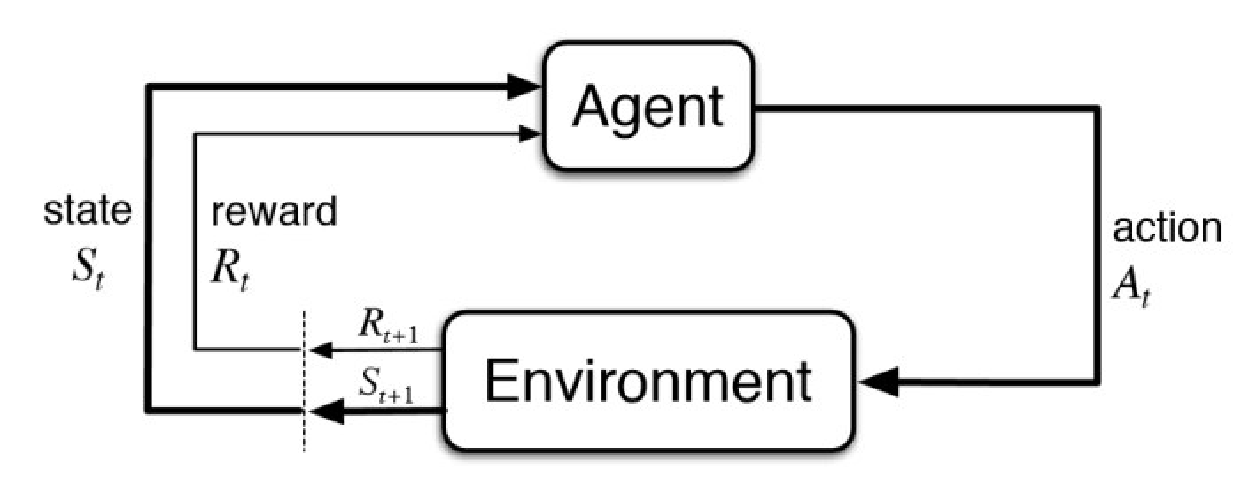
\includegraphics[width=1\textwidth]{figures/rl_general.pdf}
	\caption{Reinforcement Learning. An agent chooses an action to interact with the environment and gets a reward and an observation of his new state back. 
		\label{rl_general}	
		\cite{rl_general.jpg}
	}
\end{figure}

\vspace{0.5cm}

%policy 
In each state there is an action that the agent considers best due to its current knowledge about the expected rewards of each action. This set of actions is known as the policy 
$\pi (s)$. 
The goal of getting maximal reward can be interpreted as finding the best actions in each state that give the most reward, which is finding the optimal policy. The policy can also be either deterministic or stochastic, depending on the transition probability of the environment.

\vspace{0.5cm}

%value function
A value function is used to measure how good a state or action is. Two types of value functions are used for the states and the actions. the state value function is denoted as V(s). The value of a state is the expected reward when acting according to the policy 
$\pi$ \cite{rlwiki}.
V(s) is defined as follows in equation \ref{eq:state-value-function}.

\begin{equation}
\label{eq:state-value-function}
V^\pi (s) = \mathbb{E} [R | s,\pi]
\end{equation}

The actions value function is denoted as Q(s,a) and is defined In equation \ref{eq:action-value-function}.

\begin{equation}
\label{eq:action-value-function}
Q^\pi (s,a) = \mathbb{E} [R | s,a,\pi]
\end{equation}

When determining the value of a state or action, a discount factor $\gamma$
is used to discount future rewards towards immediate rewards. 
The idea is that a state s is not only as good as the reward you get when transitioning to that state. Future rewards from states that are reachable from state s should also be considered. The value of a state consists of the reward that you get by transitioning to that state and the potential rewards that can be gained by transitioning from that state. 
Since future rewards are not as certain as immediate rewards, the discount factor is used. The farther a reward is in the future, the more it is discounted. 
%bellman equations
The Bellman equations described in equation \ref{eq:V-bellman} and \ref{eq:Q-bellman} are a set of equations that convert the value functions into the immediate and future reward and can be used to update the value-functions \cite{rllilianweng}.

\begin{equation}
\label{eq:V-bellman}
V_\pi (s) = \sum_{a \in A}  \pi(a|s) (R(s,a) + \gamma \sum_{s' \in S} P_{ss'}^a V_\pi (s'))
\end{equation}

\begin{equation}
\label{eq:Q-bellman}
Q_\pi (s,a) = R(s,a) + \gamma \sum_{s' \in S} P_{ss'}^a \sum_{a \in A}  \pi(a'|s') Q_\pi(s',a')
\end{equation}

The goal is to find the actions that return the maximal reward. This is displayed by the Bellman optimality equations (\ref{eq:V-optbellman},\ref{eq:Q-optbellman}) \cite{rllilianweng}:

\begin{equation}
\label{eq:V-optbellman}
V_\ast (s) = \max_{a \in A} (R(s,a) + \gamma \sum_{s' \in S} P_{ss'}^a V_\ast (s'))
\end{equation}

\begin{equation}
\label{eq:Q-optbellman}
Q_\ast (s,a) = R(s,a) + \gamma \sum_{s' \in S} P_{ss'}^a \max_{a \in A} Q_\ast(s',a')
\end{equation}

To calculate the optimal values of each state and action, Dynamic Programming could be used if the entire model is known. But even knowing the entire model is not good enough as usually the main issue lies in the huge state and action space, which makes it impossible to use Dynamic Programming. For RL, artificial neural networks (ANNs) can be used to approximate the value functions \cite{neuralnetpath}. 

When following the current policy, the agent will earn the maximal reward that it could earn with current knowledge, but never more than that. To learn, the agent has to deviate from the policy and explore different actions and states. The question is how much deviation is necessary, as the agent also needs to exploit most of the policy path it has learned until now because following most of the policy has a higher probability of earning a high reward. This is known in RL as the exploration vs. exploitation problem. Usually there is a variable $\epsilon$ that determines with which probability the agent will deviate from the policy. It is set rather low to let the agent exploit most of its policy. As an example, an approach is $\epsilon$-greedy \cite{egreedy}. With a high probability of $1-\epsilon$ the agent will choose the policy and with a probability of $\epsilon$ a random action is chosen. This ensures that the agent exploits most of the policy, but also explores more possible actions that might bring more reward. 

%%neuronal networks
\section{Artificial Neural Networks}

ANNs are inspired by the human brain. 
%\nnbio, blablabla
The ANN consists of layers of neurons. Each neuron is connected to the next layer of neurons. There is one input layer and one output layer at the beginning and end of the layer of neurons. The layers between the input and output layers are called hidden layer. The hidden layer can consist of only one or more layers. The idea is to train the ANN to take inputs and produce outputs. To approximate the value functions the input would be states and actions, the output should be the correct and optimal values of these states and actions. An example of an ANN is shown in Figure \ref{neuralnet}.

\begin{figure} [h]
	\centering
	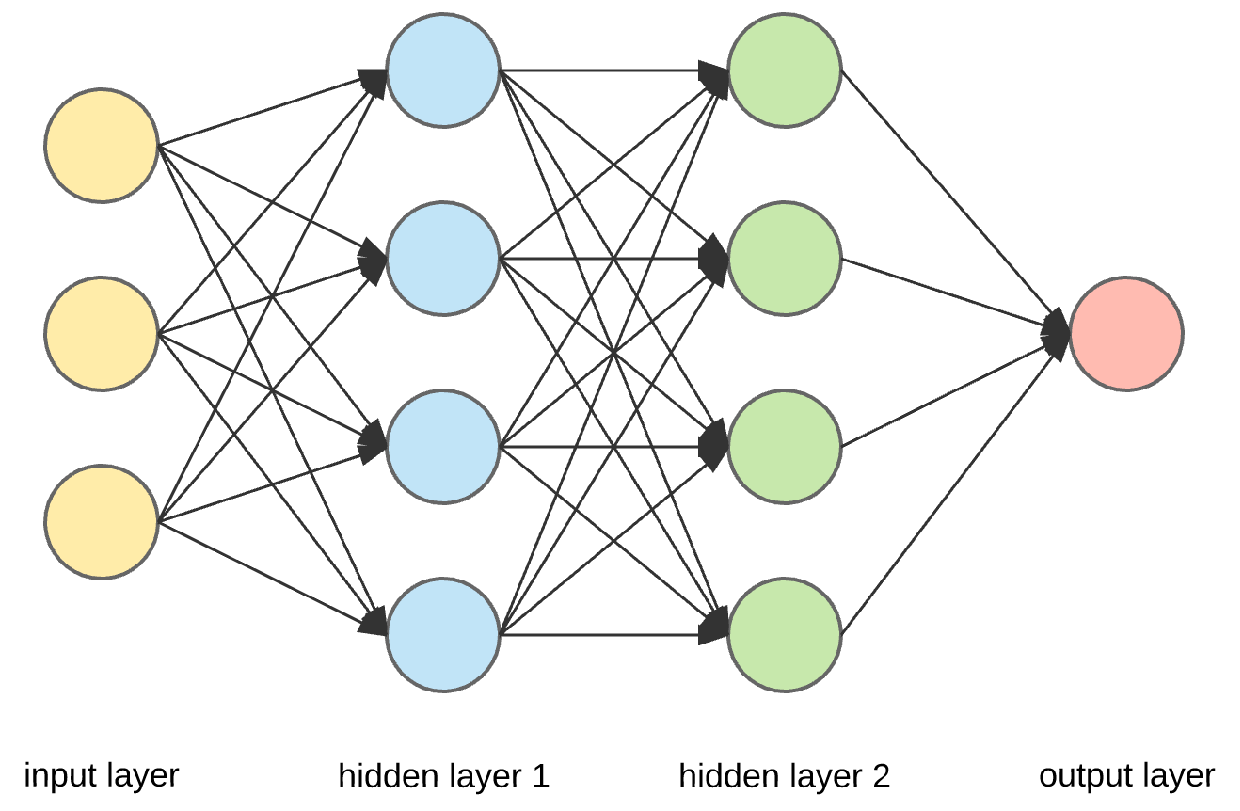
\includegraphics[width=1\textwidth]{figures/neural_network.pdf}
	\caption{A neural network. \cite{neural_networkpng}}
	\label{neuralnet}
\end{figure}

\vspace{0.5cm}

The learning process of the neuronal network is as follows. Each neuron obtains inputs $x_i$ by the the outputs of the neurons in the layer before it. Each input value is weighted and then the sum of these weighted values is taken. A bias $b$ is also added to support the learning process. After using an activation function on the sum, the value is output to the next layer of neurons. The activation function is a simple function that either reduces the output of the neuron to 0 if the value is below a certain threshold, otherwise the value is output unfiltered.
The training process of the neuron can be seen in Figure \ref{neuron}.
%besser formulieren!

\begin{figure} [h]	
	\centering
	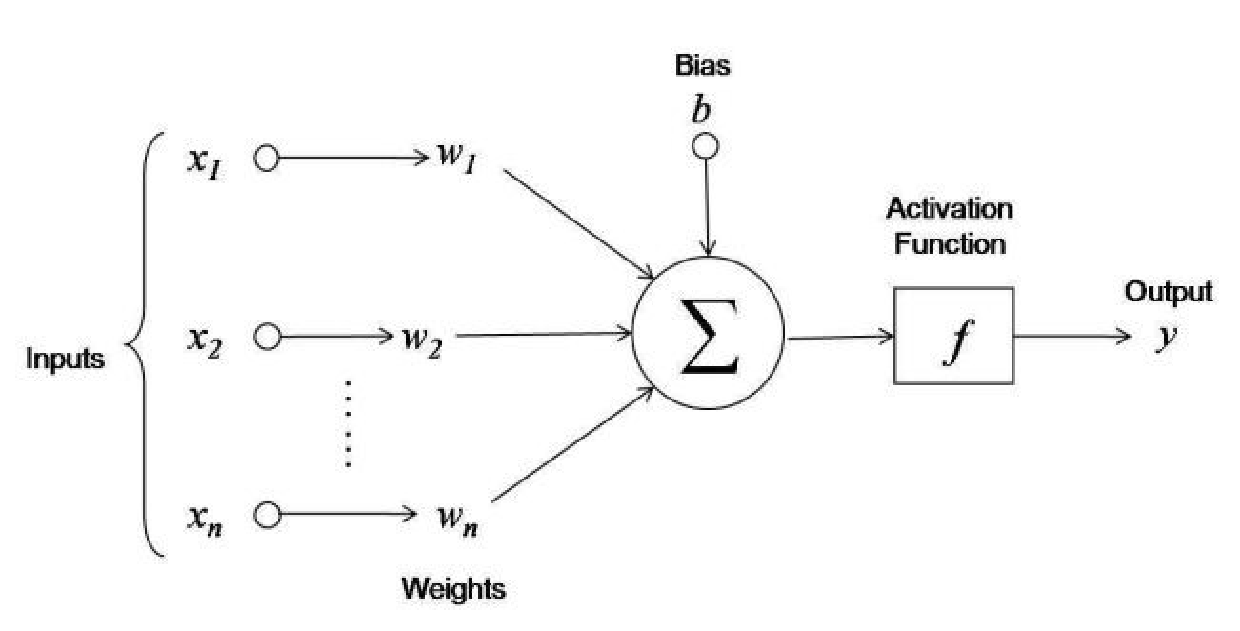
\includegraphics[width=1\textwidth]{figures/neuron.pdf}
	\caption{A neuron and how its value is composed \cite{neuron.jpeg}}
	\label{neuron}
\end{figure}

\vspace{0.5cm}

When the ANN outputs a value, a process called Backpropagation is used to improve the ANN \cite{backprop}. When initializing the ANN, the actual right weights for the input values are unknown, so random values for the weights are used. Therefore, the output values will not be right. By using an error function, the amount of error can be computed. The amount of error can be used to figure out how much the weights have to be modified for the output to become right. Backpropagation is the process of going backwards through the ANN and improving the weights of the neurons that caused the output value to be wrong. By repeating the whole process, the weight of each neuron converges towards an optimal value. 

\vspace{0.5cm}

\section{Deep Deterministic Policy Gradients}

The paper by Silver et al. is a recommended resource for more detailed explanations \cite{ddpg}. This chapter will give a short summary of DDPG.
The algorithm DDPG learns concurrently a Q-function (the action-value function) and a policy. \cite{ddpg}
Q*(s,a) is used to find the the optimal action in each state.
To compute the Q-values for a discrete action space, the Q-values of each action could be calculated and compared to find the biggest value. But in a continuous action space it is not possible to calculate the Q-value for each action. DDPG uses the fact that the action space is continuous and so Q*(s,a) is expected to be differentiable in respect to the action argument. \cite{ddpg}
This way it is possible to approximate the Q-values and policy.

\vspace{0.5cm}

To learn the Q-values, the Bellman equation for the action value is used. To approximate the Q-values, a mean squared Bellman error function is used.
The idea is that minimizing this function error is equal to approximating the current Q-values to the optimal Q-values.

\vspace{0.5cm}

For DDPG an experience replay buffer is also used. The replay buffer is a set of experiences. This can be used to replay old experiences. When only using new experiences, the ANN might be overfit to those experiences. Being overfit means that for some experiences the ANN will output very good results, but for most other experiences it will perform very bad. Experience replay is useful to prevent that. But a too large buffer can cause the learning process to slow down. The right balance has to be found.

DDPG also uses target networks. Equation \ref{eq:target} is called target \cite{ddpg}.

\begin{equation}
\label{eq:target}
r + \gamma (1-d) \max_{a'} Q_\phi(s',a')
\end{equation}

The target is what is desired for the Q-function to approximate to.
When minimizing the mean squared bellman error function, there is the problem that the target is also dependent on the parameters that are trained. When changing the parameters, the target would also change which is problematic. That is why the target network, a copy of the ANN is used. The update of the target network is delayed to avoid this conflict.
To find the optimal policy, simply gradient ascent can be used to find the maximal Q-values.


\section{Hindsight Experience Replay}

%subsection curriculum learning ?

%read paper, use it
Sparse rewards are a big issue in RL, especially in tasks for robotic arms often the rewards are sparse. Having sparse rewards means that most of the samples used for training will not successful and therefore will not bring any useful reward. For example, the task to move an object to a certain point would have a sparse reward for a robotic arm because very precise movements are needed which the robotic arm has to learn first.
 
\vspace{0.5cm}
 
Andrychowicz et al. have shown that HER can be used to deal with this issue for robotic arms \cite{herpaper}
HER can learn efficiently from sparse rewards and can also be combined with any off-policy RL algorithm.
This technique is inspired by the ability of humans to learn from failures as least as much as from successes.

\vspace{0.5cm}

HER works as follows. After an episode of gaining experiences, all transitions between the states in each training sample is stored in a replay buffer, but the goal that was not achieved is extended to a set with a goal that is reached. This can also be further extended to a set of more goals that can be achieved in the terminating state of the training sample. If the goal was to move an object to point x, but it was pushed to point y, the replay buffer would use the same transitions but change the the goal we wanted to achieve to y. So when replaying the same experience, the agent would be successful and earn an useful reward. This does not help the agent learn how to reach the goal it wanted to reach initially, but it learns how to reach other goals. Being able to reach those other already achieved goals might be beneficial in learning how to reach the goal it actually wanted to achieve. HER is mainly used for tasks with multiple goals, but it was shown that it also improves the training of tasks with only a single goal. \cite{herpaper}
Interestingly, Andrychowicz et al. have shown HER performs has problems when using shaped rewards. \cite{herpaper}
%add binary rewards at start of section ?. binary != shaped ?
 
 %add pseudocode ?

		
		\chapter{Methodology}


\section{Simulation Environment}

This section describes the environment and tools used for the experiments.

MuJoCo is a physics engine used to simulate the physical models of the environment. MuJoCo is currently still in development and is improved, so there are many different versions. For this thesis, MuJoCo 2.0 for Linux (Ubuntu 16.04) is used. 
\newline
mujoco-py is used as an interface to allow the usage of MuJoCo in python scripts. mujoco-py is required for OpenAI Gym to work.
\newline
OpenAI developed OpenAI Gym, a toolkit to create and use environments, and use these environments to test and compare algorithms for RL. OpenAI Gym only provides the environment part of RL, the agent has to be written by the user or by using OpenAI baselines. The robotic environments require MuJoCo. In our case, we will create our own environments and compare them to the existing ones.
\newline
OpenAI baselines is a toolkit with high-quality implementations of RL algorithms. It supplements the OpenAI Gym toolkit. For each of the environments by OpenAI Gym, any OpenAI baselines RL algorithm can be used. In our case, we will focus mainly on HER.
\newline
All the experiments will run on a 12 core machine using 10 cores. The machine is running on the operating system Linux Ubuntu 16.04. The parameters used are listed in the appendix. If not otherwise specified, each experiment will be run for 50 episodes. which takes about 2 hours of training time each.


\subsection{MuJoCo}
%physic engine, modeling, mujoco-py for python interface

%mujco is free (no costs) for non-profit research ?
MuJoCo stands for "Multi-Joint dynamics with Contact". It is a physics engine for model based control and was developed by Todorov et al. \ref{mujoco}.
MuJoCo was developed for research in areas with fast and accurate simulation, like robotics. As its name suggests, multi-joint dynamics and contact responses and contact responses are a main focus of the engine. They represented multi-joint dynamics in generalized coordinates and computed them with recursive algorithms. For the contact responses, they wrote algorithms based on a modern velocity-stepping approach. MuJoCo was developed to be fast and accurate, especially for computationally intensive processes, which are common in simulations of physics. 
\newline
Todorov et al. compared MuJoCo to SD/FAST, another tool to simulate physics of mechanical systems. Even though SD/FAST uses model-specific code, which was expected to be much fast, MuJoCo was quite comparable. Their tests with a 12-core machine showed 400.000 dynamics evaluations per second for a 3D humanoid with 18 DOF and 6 active contacts. 
Creating models for MuJoCo is quite simple. For MuJoCo, XML files can be used, which are simple to understand and provide high transparency. 
%explain more how to do xml for mujoco ? - no
\newline
To use MuJoCo with Python, mujoco-py was created by OpenAI. Mujoco-py currently supports compatibility of MuJoCo with Python 3.

\subsection{OpenAI}
OpenAI developed OpenAI Gym and OpenAI Baselines. Both are freely accessible on Github.

\subsubsection{OpenAI Gym}
%environments
OpenAI Gym provides an environment to test a RL algorithm with. OpenAI Gym already contains many environments to use, like Atari games, classic control problems and robotics. In this thesis, the robotics environment will be used, as it provides four environments with fetch robots that use a robotic arm. But OpenAI also allows the user to create his own environments. For the experiments, a few more robotics environments will be created. For the robotics environments MuJoCo is required. 
The agent and the RL algorithms that are required for RL to interact with the environment have to be either coded by the user or provided by OpenAI Baselines.

\subsubsection{OpenAI Baselines}
%algorithms
OpenAI Baselines provides a set of high-quality implementations of RL algorithms. It can be used together with OpenAI Gym. Provided algorithms contain Advantage Actor Critic, Actor critic with experience replay, Actor Critic using Kronecker-Factored Trust Region, DDPG, Deep Q-Networks, Generative Adversarial Imitation Learning, Proximal Policy Optimization, Trust Region Policy Optimization and HER.
For our purposes, HER in conjunction with DDPG will be used. 
OpenAI Baselines also requires Tensorflow to work.

\section{Model}
%Explain general things like action space etc. of the robot. sucess rate etc.

\begin{figure} [h]
	\centering
	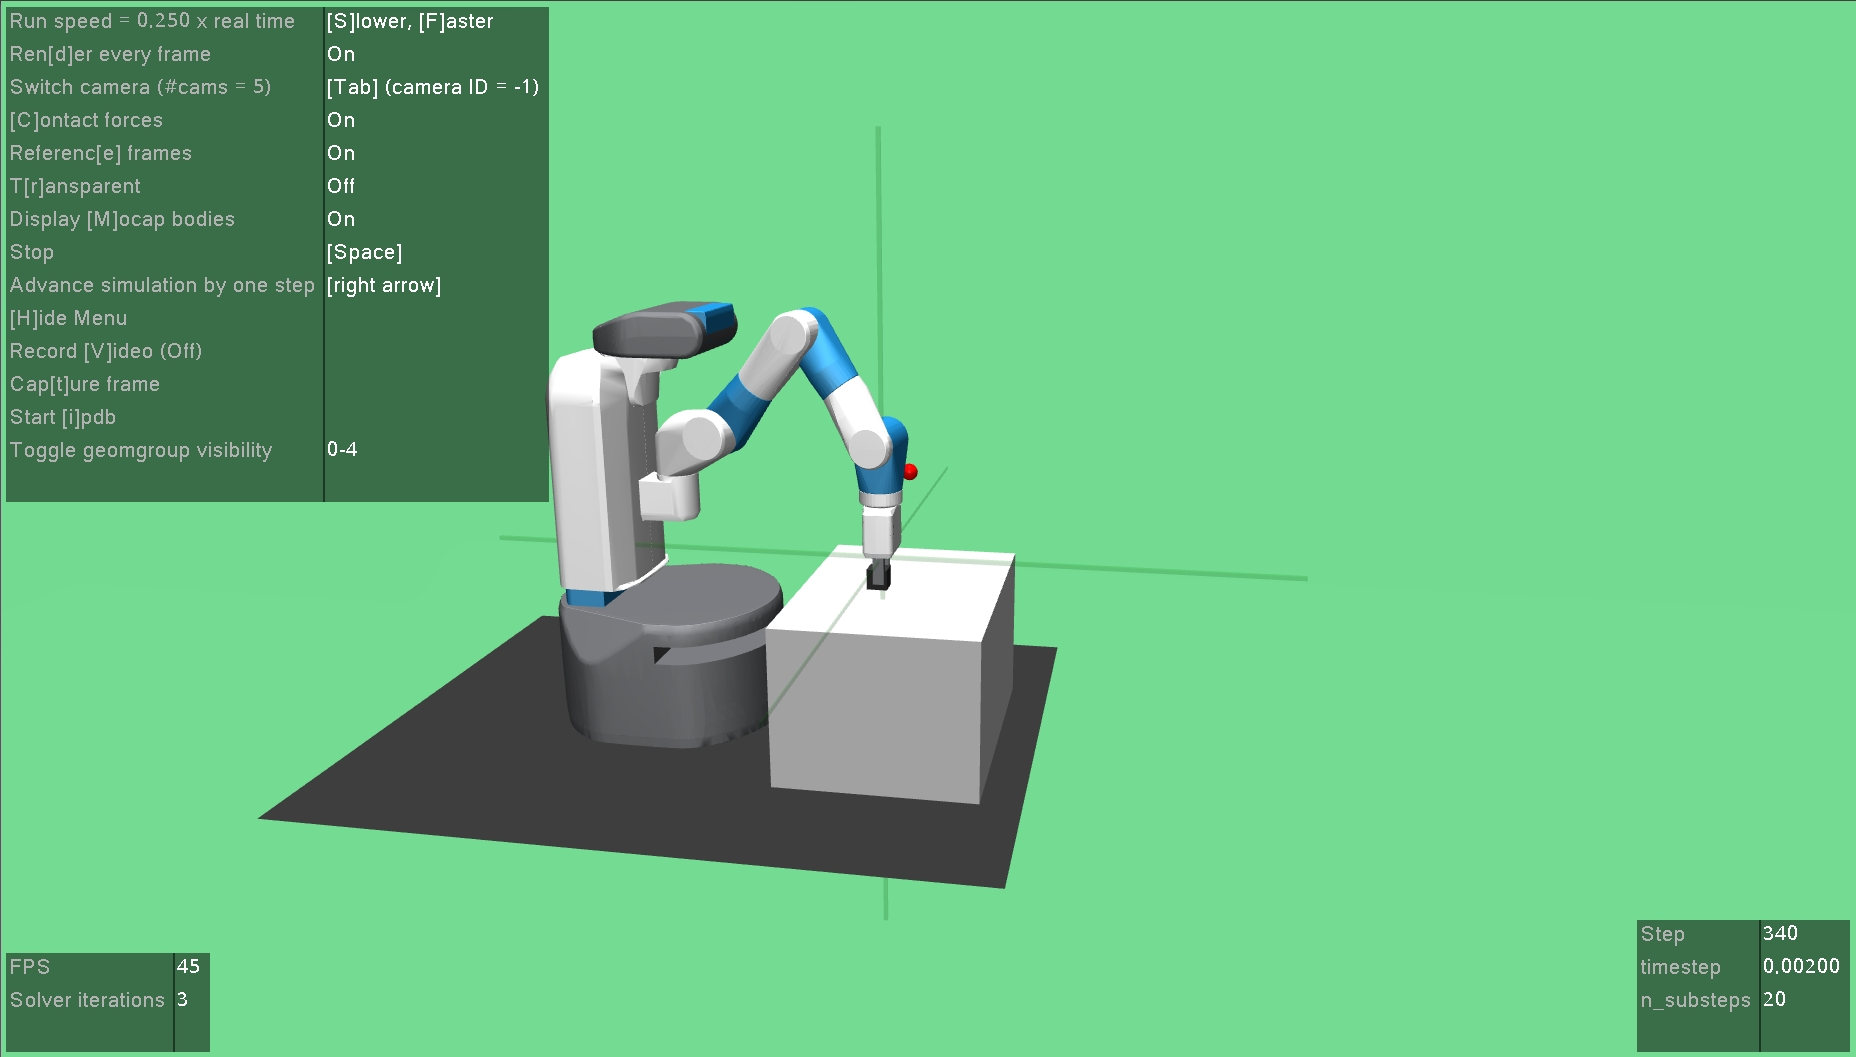
\includegraphics[width=1\textwidth]{figures/FetchPickAndPlace-v1.png}
	\caption{the FetchPickAndPlace-v1 environment by OpenAI Gym run with mujoco-py}
	\label{pickplace1}
\end{figure}

The environment model used is quite simple. The environments are the basic fetch environments in the robotics environment package of OpenAI gym \cite{plappert}, for the extended harder experiments, the object is changed to a ball. Otherwise, only positions of the object and goal as well as properties like size and friction are changed.

\vspace{0.5cm}

In figure \ref{pickplace1} the environment for the task "FetchPickAndPlace" by OpenAI is shown. A fetch robotic arm with 7 DOF is used. Its end effector is a two-fingered parallel gripper. Even though it is simulated in MuJoCo, Andrychowicz et al. have shown in their paper on HER, that the robotic arm also performed well in real life without any finetuning \ref{herpaper}. 

\vspace{0.5cm}

All the tasks require an object (either a cube or a ball) to be moved to a goal that is presented by a red point. Also a table is used to increase the height of the object and goal, so the fetch robot can grab the object.
Some parameters except from position parameters that might differ depending on the robotics environment are listed here.

\begin{itemize}
	\item has\_object (boolean): describes whether the environment contains an object or not
	\item block\_gripper (boolean): if True, the fetch robot can not open or close its gripper
	\item n\_substeps (integer): number of timesteps before the next action is chosen
	\item target\_in\_the\_air (boolean): if True, the target is is not on the ground or table 
	\item object\_range (float): defines a range in which the object will be randomly and uniformly placed
	\item target\_range (float): defines the range in which the goal will be randomly and uniformly placed
	\item distance\_threshold (float): the distance the object can be to the goal for the goal to be still successful 
\end{itemize}

In RL, the agent chooses an action and receives a reward and an observation after each step. actions, rewards and observations are handled in OpenAI Gym as follows.

\begin{itemize}
	\item Action: The action space is defined as a 4-dimensional Box space, which is an array of 4 floats, which are continuous and between -1 and 1. The 4 floats define how to change the x-position, y-position and z-position of the gripper and how much to open/close the gripper (if the parameter block\_gripper is False)
	\item Reward: The reward defined as a float. In the robotics environments, the agent receives a reward of -1.0 in each timestep, in which the goal is not reached.
	\item Observation: The observation space contains 3 parts:
	the achieved\_goal, defined by a 3-dimensional Box space, which is useful for HER. 
	the desired\_goal, also defined by a 3-dimensional Box space.
	the observation: defined by a 25-dimnsional Box space
\end{itemize}

If not stated otherwise, each environment sample will be run for 50 steps. With the number of substeps being usually fixed to 20, each sample will run for 1000 timesteps. 
%%use this stuff if it fits


		
		%\chapter{Simulation Environment}

This section describes the environment and tools used for the experiments.

MuJoCo is a physics engine used to simulate the physical models of the environment. MuJoCo is currently still in development and is improved, so there are many different versions. For this thesis, MuJoCo 2.0 for Linux (Ubuntu 16.04) is used. 

\vspace{0.5cm}

Mujoco-py is used as an interface to allow the usage of MuJoCo in python scripts. Mujoco-py is required for OpenAI Gym to work.

\vspace{0.5cm}

OpenAI developed OpenAI Gym, a toolkit to create and use environments, and use these environments to test and compare algorithms for reinforcement learning. OpenAI Gym only provides the environment part of reinforcement learning, the agent has to be written by the user or by using OpenAI baselines. The robotic environments require MuJoCo. In our case, we will create our own environments and compare them to the existing ones.

\vspace{0.5cm}

OpenAI baselines is a toolkit with high-quality implementations of reinforcement learning algorithms. It supplements the OpenAI Gym toolkit. For each of the environments by OpenAI Gym, any OpenAI baselines reinforcement learning algorithm can be used. In our case, we will focus mainly on Hindsight Experience Replay.

\vspace{0.5cm}

All the experiments will were done on a 12 core machine using 10 cores. The machine is running on the operating system Linux Ubuntu 16.04. The parameters used will be stated in the Model section. If not otherwise specified, each experiment will be run for 50 episodes. which takes about 2 hours training time each.


\section{MuJoCo}
%physic engine, modeling, mujoco-py for python interface

%mujco is free (no costs) for non-profit research ?
MuJoCo stands for "Multi-Joint dynamics with Contact". It is a physics engine for model based control and was developed by Emanuel Todorov.
%ref Mujoco paper
MuJoCo was developed for research in areas with fast and accurate simulation, like robotics. As its name suggests, multi-joint dynamics and contact responses and contact responses are a main focus of the engine. They represented multi-joint dynamics in generalized coordinates and computed them with recursive algorithms. For the contact responses, they wrote algorihhms based on a modern velocity-stepping approach. MuJoCo was developed to be fast and accurate, especially for computationally intensive processes, which are common in simulation of physics. 

\vspace{0.5cm}

They compared MuJoCo to SD/FAST, another tool to simulate physics of mechanical systems. Even though SD/FAST uses model-specific code, which was expected to be much fast, MuJoCo was quite comparable. Their tests with a 12-core machine showed 400.000 dynamics evaluations per second for a 3D humanoid with 18 Degrees of Freedom and 6 active contacts. 
Creating models for MuJoCo is quite simple. For MuJoCo, XML files can be used, which are simple to understand and provide transparency. 
%explain more how to do xml for mujoco ?

\vspace{0.5cm}

To use MuJoCo with Python, mujoco-py was created by OpenAI. Mujoco-py currently supports compatibility of MuJoCo with Python 3.



\section{OpenAI}

OpenAI developed OpenAI Gym and OpenAI Baselines. Both are freely accessible on Github.


\subsection{OpenAI Gym}
%environments

OpenAI Gym provides an environment to test a reinforcement learning algorithm with. OpenAI Gym already contains many environments to use, like Atari games, classic control problems and robotics. In this thesis, the robotics environment will be used, as it provides four environments with Fetch robots that use a robotic arm. But OpenAI also allows the user to create his own environments. For the experiments, a few more robotics environments will be created. For the robotics environments, MuJoCo is required. 
The agent and the reinforcement learning algorithms it uses that are required for reinforcement learning to interact with the environment has to be either written by the user or provided by OpenAI Baselines.

\subsection{OpenAI Baselines}
%algorithms

OpenAI Baselines provides a set of high-quality implementations of reinforcement learning algorithms. It can be used together with OpenAI Gym. Provided algorithms contain Advantage Actor Critic, Actor critic with experience replay, Actor Critic using Kronecker-Factored Trust Region,  Deep Deterministic Policy Gradient, Deep Q-Networks, Generative Adversarial Imitation Learning, Proximal Policy Optimization, Trust Region Policy Optimization and Hindsight Experience Replay.
For our purposes, Hindsight Experience Replay in conjunction with Deep Deterministic Policy Gradients will be used. 
OpenAI Baselines also requires Tensorflow to work.

\section{Model}
%Explain general things like action space etc. of the robot. sucess rate etc.

\begin{figure} [h]
	
	\centering
	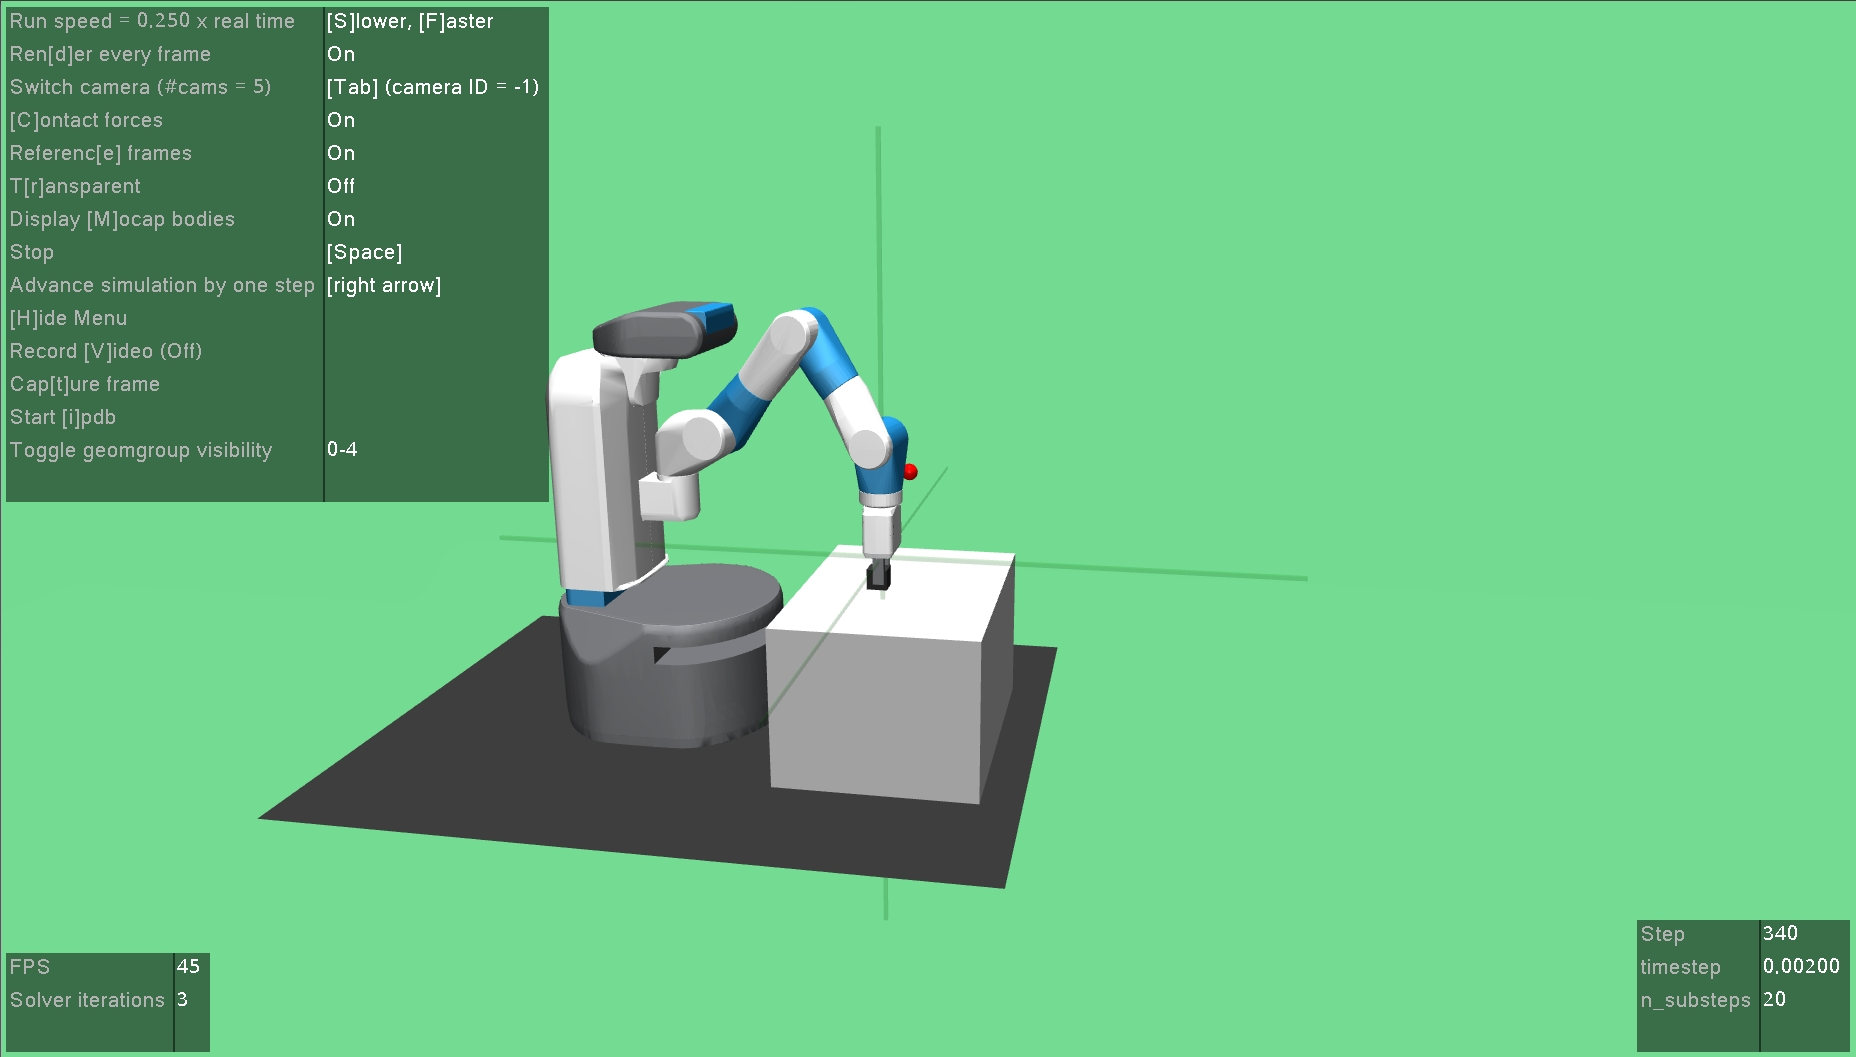
\includegraphics[width=1\textwidth]{figures/FetchPickAndPlace-v1.png}
	\caption{FetchPickAndPlace-v1 Environment by OpenAI Gym run with Mujoco-py
	}
\end{figure}

The environment model used is quite simple. The environments are the basic models in the robotics environment package of OpenAI gym, for the extended harder experiments, only positions of the objects and goal, and properties like size and friction are changed. 
%ref https://openai.com/blog/ingredients-for-robotics-research/

\vspace{0.5cm}

In figure 4.1. the environment for the FetchPickAndPlace task of OpenAI is shown. A Fetch Robotic arm with 7 Degrees of Freedom is used. Its end effector is a two-fingered parallel gripper. Even though it is simulated in MuJoCo, Andrychowicz et al. have shown in their paper on Hindsight Experience Replay, that the robotic arm also performed well in real life without any finetuning. 
%ref herpaper

\vspace{0.5cm}

All the tasks require an object (either a cube or a ball) to be moved to a goal that is presented by a red point. Also a table is used to increase the height of the object and goal, so the fetch robot can grab the object.
Some parameters except from position parameters that might differ depending on the robotics environment are listed here.

\begin{itemize}
	\item has\_object (boolean): describes whether the environment contains an object or not
	\item block\_gripper (boolean): if True, the fetch robot can not open or close its gripper
	\item n\_substeps (integer): number of timesteps before the next action is chosen
	\item target\_in\_the\_air (boolean): if True, the target is is not on the ground or table 
	\item object\_range (float): defines a range in which the object will be randomly and uniformly placed
	\item target\_range (float): defines the range in which the goal will be randomly and uniformly placed
	\item distance\_threshold (float): the distance the object can be to the goal for the goal to be still successful 
\end{itemize}

In Reinforcement Learning, the agent chooses an action and receives a reward and an observation after each step. Actions, Rewards and Observations are handled in OpenAI Gym as follows.

\begin{itemize}
	\item Action: The action space is defined as a 4-dimensional Box space, which is an array of 4 floats, which are continuous and between -1 and 1. The 4 floats define how to change the x-position, y-position and z-position of the gripper and how much to open/close the gripper (if the parameter block\_gripper is False)
	\item Reward: The reward defined as a float. In the robotics environments, the agent receives a reward of -1.0 in each timestep, in which the goal is not reached.
	\item Observation: The observation space contains 3 parts:
	the achieved\_goal, defined by a 3-dimensional Box space, which is useful for Hindsight Experience Replay. 
	the desired\_goal, also defined by a 3-dimensional Box space.
	the observation: defined by a 25-dimnsional Box space
\end{itemize}




If not stated otherwise, each environment sample will be run for 50 steps. With number of substeps being usually fixed to 20, each sample will run for 1000 timesteps. The hyperparameters are as follows for each of the following environments:
%TODO
%%use this stuff if it fits, parameters (PickPlace)

%T: 50
%_Q_lr: 0.001
%_action_l2: 1.0
%_batch_size: 256
%_buffer_size: 1000000
%_clip_obs: 200.0
%_hidden: 256
%_layers: 3
%_max_u: 1.0
%_network_class: %baselines.her.actor_critic:ActorCritic
%_norm_clip: 5
%_norm_eps: 0.01
%_pi_lr: 0.001
%_polyak: 0.95
%_relative_goals: False
%_scope: ddpg
%aux_loss_weight: 0.0078
%bc_loss: 0
%ddpg_params: {'layers': 3, 'polyak': 0.95, 'Q_lr': 0.001, 'hidden': 256, 'norm_eps': 0.01, 'batch_size': 256, 'pi_lr': 0.001, 'buffer_size': 1000000, 'norm_clip': 5, 'clip_obs': 200.0, 'max_u': 1.0, 'network_class': 'baselines.her.actor_critic:ActorCritic', 'relative_goals': False, 'action_l2': 1.0, 'scope': 'ddpg'}
%demo_batch_size: 128
%env_name: FetchPickAndPlace-v1
%gamma: 0.98
%make_env: <function %prepare_params.<locals>.make_env at 0x7f67a97242f0>
%n_batches: 40
%n_cycles: 50
%n_test_rollouts: 10
%noise_eps: 0.2
%num_demo: 100
%prm_loss_weight: 0.001
%q_filter: 0
%random_eps: 0.3
%replay_k: 4
%replay_strategy: future
%rollout_batch_size: 2
%test_with_polyak: False
%Creating a DDPG agent with action space 4 x 1.0...

		
		\chapter{Experiments}
%Basic Environments, PickPlace is harder than reach etc., Plappert et. al., HER paper..

This chapter describes the experiments that were carried out and their results. This chapter is divided into 3 subchapters.
%change number of chapters if it changes
\newline
First the four robotics environments "FetchReach", "FetchPush", "FetchSlide" and "FetchPickAndPlace" that are already integrated in OpenAI Gym, will be compared and used as benchmarks.
%ref Plappert et al.
Then two self created environments, FetchSlideball and FetchToss will be described.
\vspace{0.5cm}

"FetchSlideball" is an extension of FetchSlide. We changed the object from a cylinder to a ball and increased the distance to the goal. This will be compared with the FetchSlide environment of the benchmarks. It is planned to improve this environment to an environment that simulates a golf course in the future.
\vspace{0.5cm}

"FetchToss" requires the agent to toss an object to a goal that is outside of the agents reach. It requires the agent to grab the object and then find the right trajectory to move the object and release it to toss it. The first part of the task is comparable to FetchPickAndPlace that requires the fetch robot to fetch the object. It was planned to improve this environment to make it toss a ball into a basket like in basketball.
\vspace{0.5cm}

In each chapter, the tasks and environment will be described. The action space, observation space and rewards to control the agent are also described. Then the results are discussed and compared to other tasks.   

%We want to have golf/basketball , so we use a ball instead
%We change the distance
%doesnt work because too far, maybe also reasons from HGG
%change friction
%interesting results, cheating v9
%use v9 on v2 is not bad, show v5
%(do v9 with wall)
%basketball
%throwing, doesnt work, too hard
%throwing ball also
%put wall, maybe it throws over goal
%try longer timesteps
%try putting box closer

\section{Fetch environments by OpenAI}

In this section, the four basic robotics environments of OpenAI with the fetch robotic arm are shortly described and compared.

\subsection{FetchReach}

\begin{figure} [h]
	
	\centering
	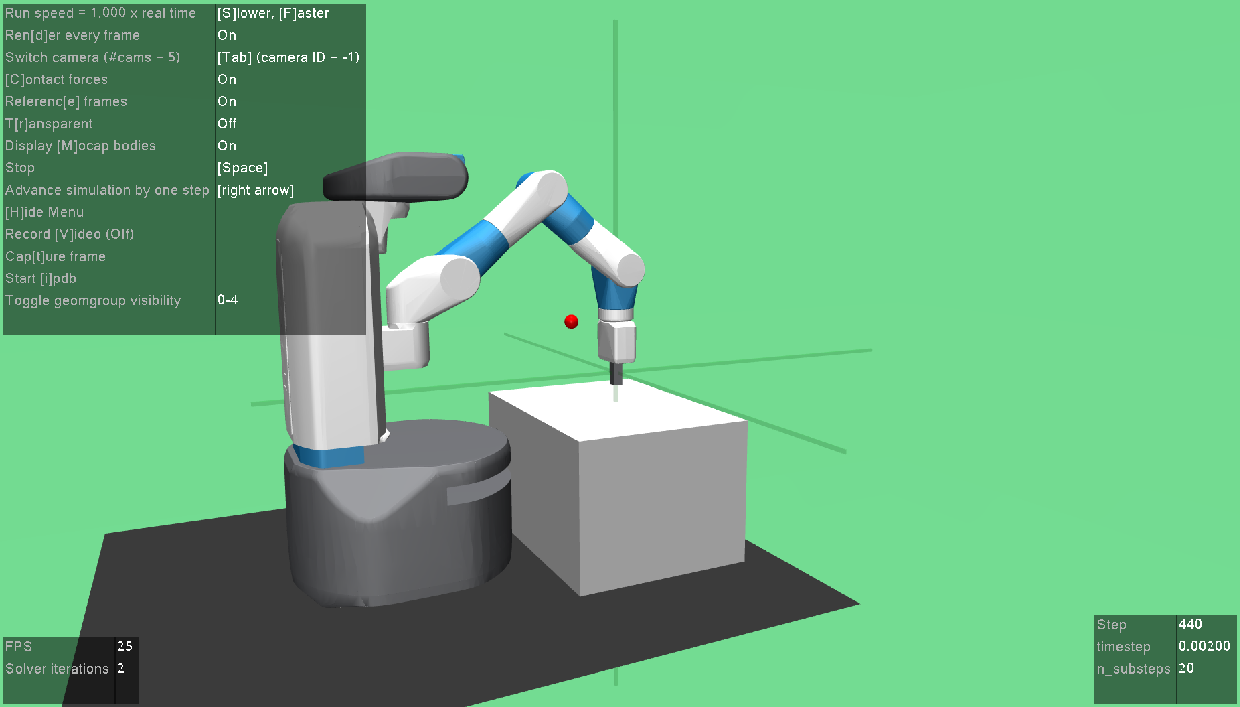
\includegraphics[width=1\textwidth]{figures/FetchReach-v1.pdf}
	\caption{FetchReach-v1}
	\label{reach1}
\end{figure} 

The environment FetchReach is the simplest of the OpenAI robotic environments. As can be seen in figure \ref{reach1}, the environment consists of the fetch robot, a table and a red ball indicating the goal. The task is to make the robot move its gripper to the same position as the goal. The goal can be on the table as well as in the air. Also, the goal is only above the table, so the robot is always able to reach the goal. The only thing the robot has to figure out is a path from one starting point to different points.

\vspace{0.5cm}

Figure \ref{benchm} shows how effective HER is.  After just about 7 epochs, the success rate is already at 100\%.




\subsection{FetchPush}

\begin{figure} [h]
	
	\centering
	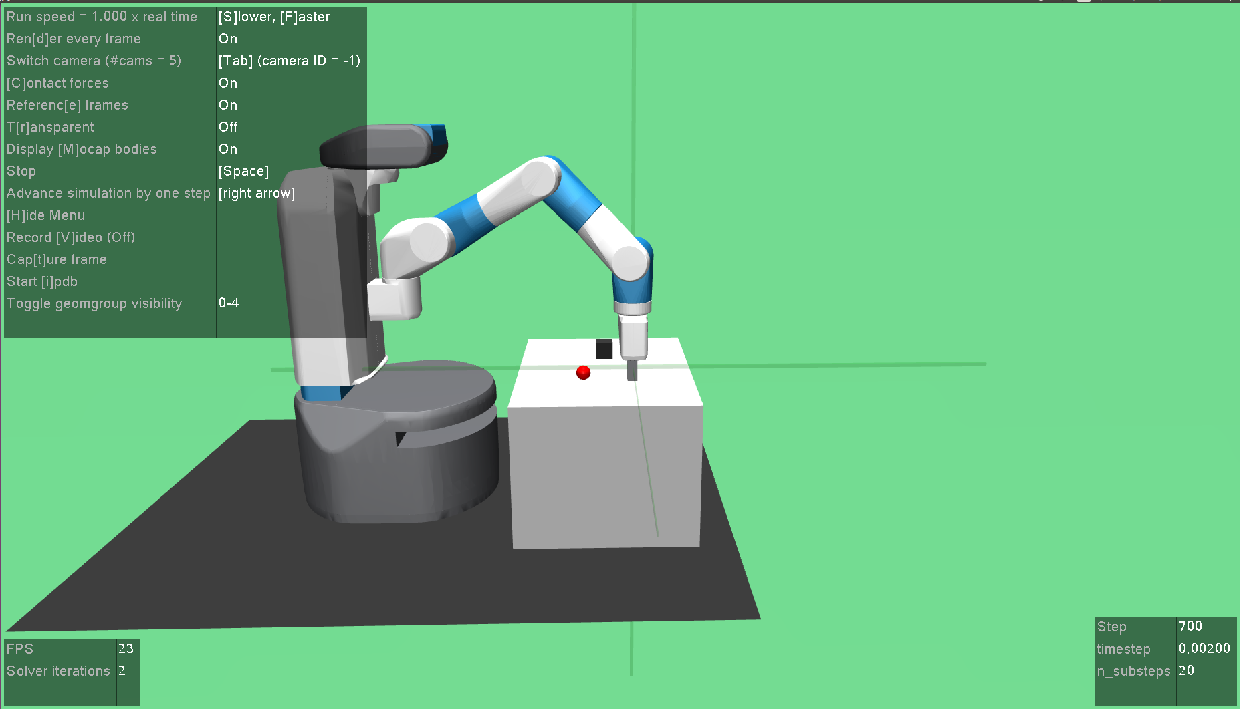
\includegraphics[width=1\textwidth]{figures/FetchPush-v1.pdf}
	\caption{FetchPush-v1}
	\label{push1}
\end{figure}

FetchPush is already much harder than FetchReach. The environment is the same as in FetchReach, but an object in form of a cube was added. This can be seen in figure \ref{push1}. The goal is to move the cube to the goal position. This requires the robot to learn how to move its gripper from the start position to the side of the cube that is away from the goal. Then it needs to move its gripper towards the goal to solve the task. Still, HER proves to be quite powerful. After about 14 epochs, In comparison to FetchReach, it took about twice the time to learn to solve the task.





\subsection{FetchSlide}

\begin{figure} [h]
	
	\centering
	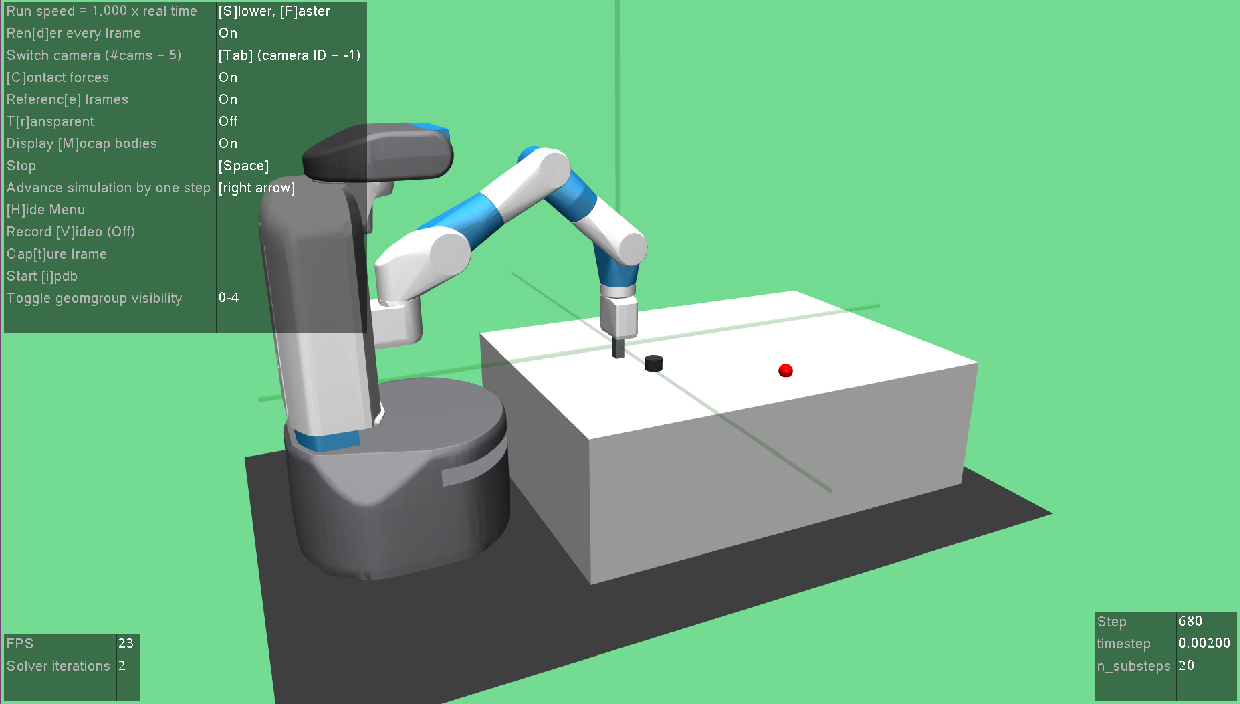
\includegraphics[width=1\textwidth]{figures/FetchSlide-v1.pdf}
	\caption{FetchSlide-v1}
	\label{slide1}
\end{figure}

The FetchSlide environment is quite similar to FetchPush. The task is the same, the robot has to move an object, this time it is a cylinder (similar to a curling stone for curling). There are two main differences to FetchPush which make the task harder. The cylinder has less friction and slides, so the robot needs to carefully move the cylinder to avoid making it slide too far. Also the goal position is further away, partly even outside of the robotic arms' range. So the sliding property of the cylinder has to be used in order to reach those goals. 

\vspace{0.5cm}

Using HER provides worse results than FetchPush. After training, the robot only reaches a success rate of about 60\%. 
In the failed attempts the robot learned to push the cylinder in the right direction, only the distance is not right. The cylinder either slides too far or does not slide far enough. Most of these fails have goal positions that are outside of the robotic arms' range. Interestingly, the robot also struggles with goals that are inside of the robotic arms' range. This is probably due to the sliding property. When touching the cylinder while training, the cylinder will probably slide further away and might often land outside of the robotic arms' reach. With HER, the agent learns to reach the states that it already reached at some point. Because the cylinder has a lot more positions it can be in due to its sliding property, other than in FetchPush, it does not learn to move the cylinder inside its range as well as in FetchPush.    

\subsection{FetchPickAndPlace}

\begin{figure} [h]
	
	\centering
	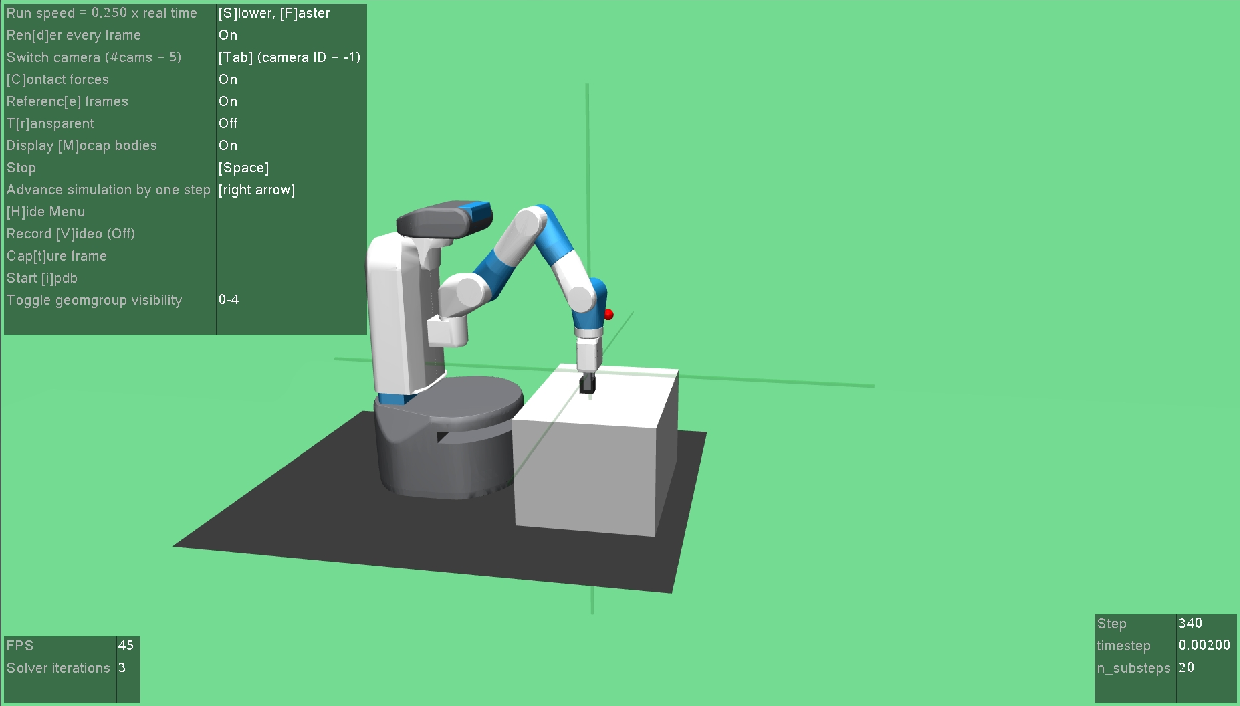
\includegraphics[width=1\textwidth]{figures/FetchPickAndPlace-v1.pdf}
	\caption{FetchPickAndPlace-v1}
	\label{pickplace2}
\end{figure}

The environment for FetchPickAndPlace is exactly the same as in FetchPush except for the goal position. It can also be in the air. This requires the robot to use its gripper to fetch the cube and move it to the goals in the air. So the robot has to learn how to move its gripper towards the cube and open its gripper, then close its gripper to grab the cube. Then it has to move the cube to the goal position without dropping the cube by opening its gripper. 
The training results in figure \ref{benchm} show that learning to solve this task works quite well with HER. After about 30 epochs it almost reaches 100\% success rate. 
%maybe in comparison part
The reason why it takes much more times than the FetchPush task can be explained when comparing both. In the FetchPush task, the agent needs to learn to move its arm to the cube on the side farther away from the goal, then move its arm towards the goal. We have seen in FetchReach that it is quite simple to learn how to move the arm from one position to another. The difficulty in FetchPush comes from figuring out how to move the object. In FetchPickAndPlace this is even harder, because the opening and closing the gripper is also part of the actions it can take. Learning how to grab the cube and keep it grabbed seems to be a the cause to why it takes more time to learn. 


\subsection{Discussion of Results}
%obv. harder tasks take longer and are performing worse
%use Plappert et. al /her paper as reference

\begin{figure} [h]
	
	\centering
	\subfigure[FetchReach-v1] {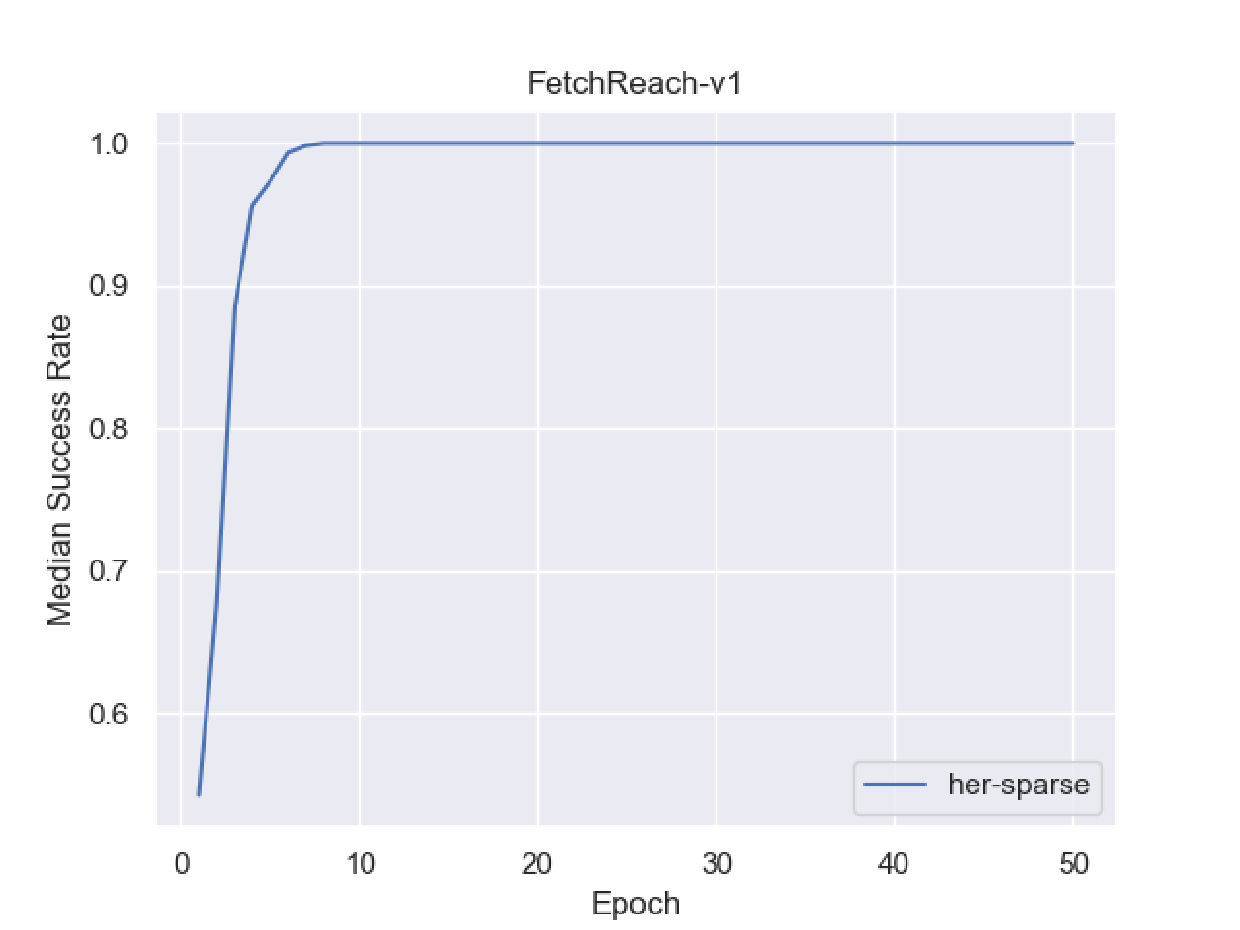
\includegraphics[width=0.49\textwidth]{figures/fig_FetchReach-v1.pdf}\label{fig:fig_fetchreach-v1}}
	\subfigure[FetchPush-v1] {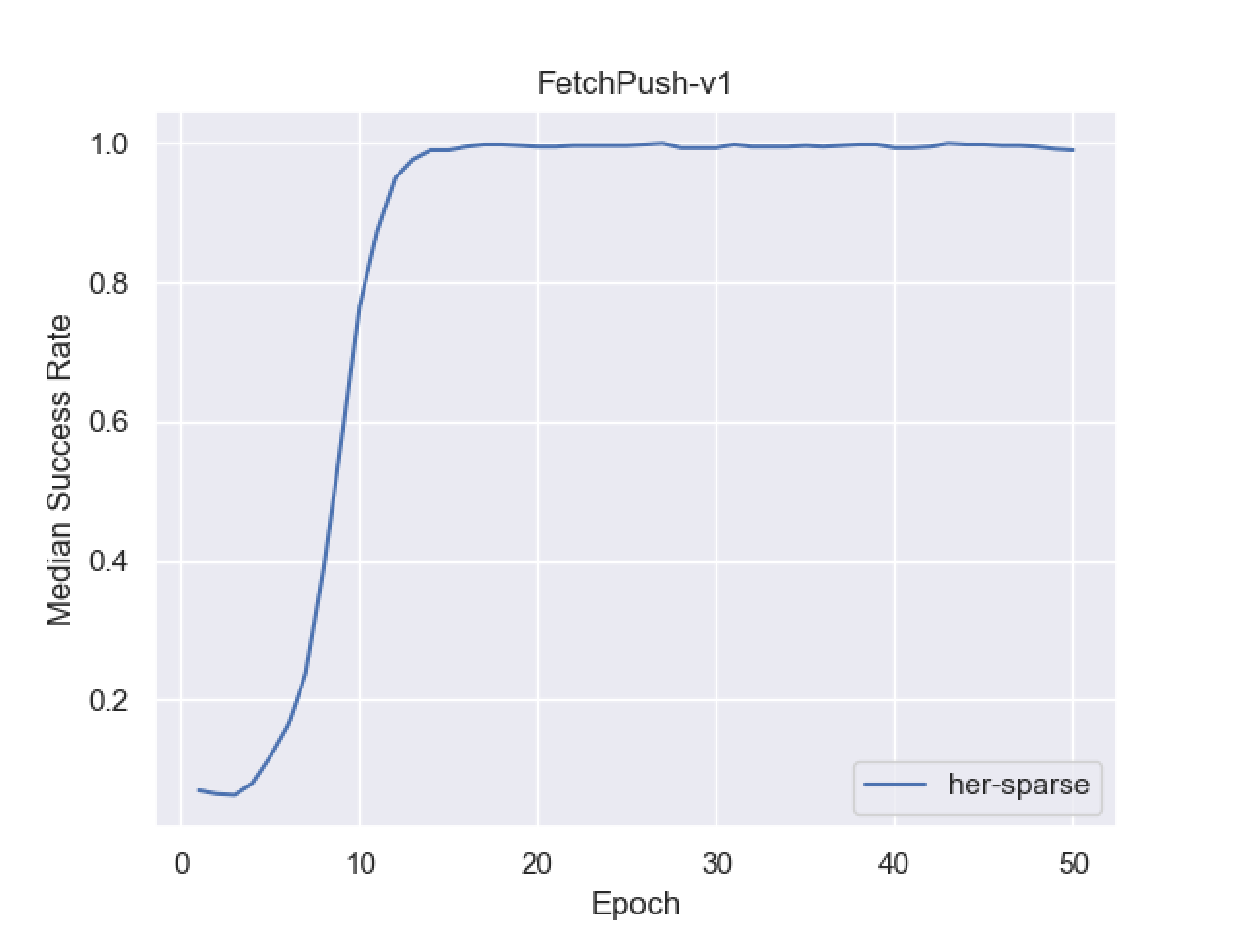
\includegraphics[width=0.49\textwidth]{figures/fig_FetchPush-v1.pdf}\label{fig:fig_fetchpush-v1}}
	\subfigure[FetchSlide-v1] {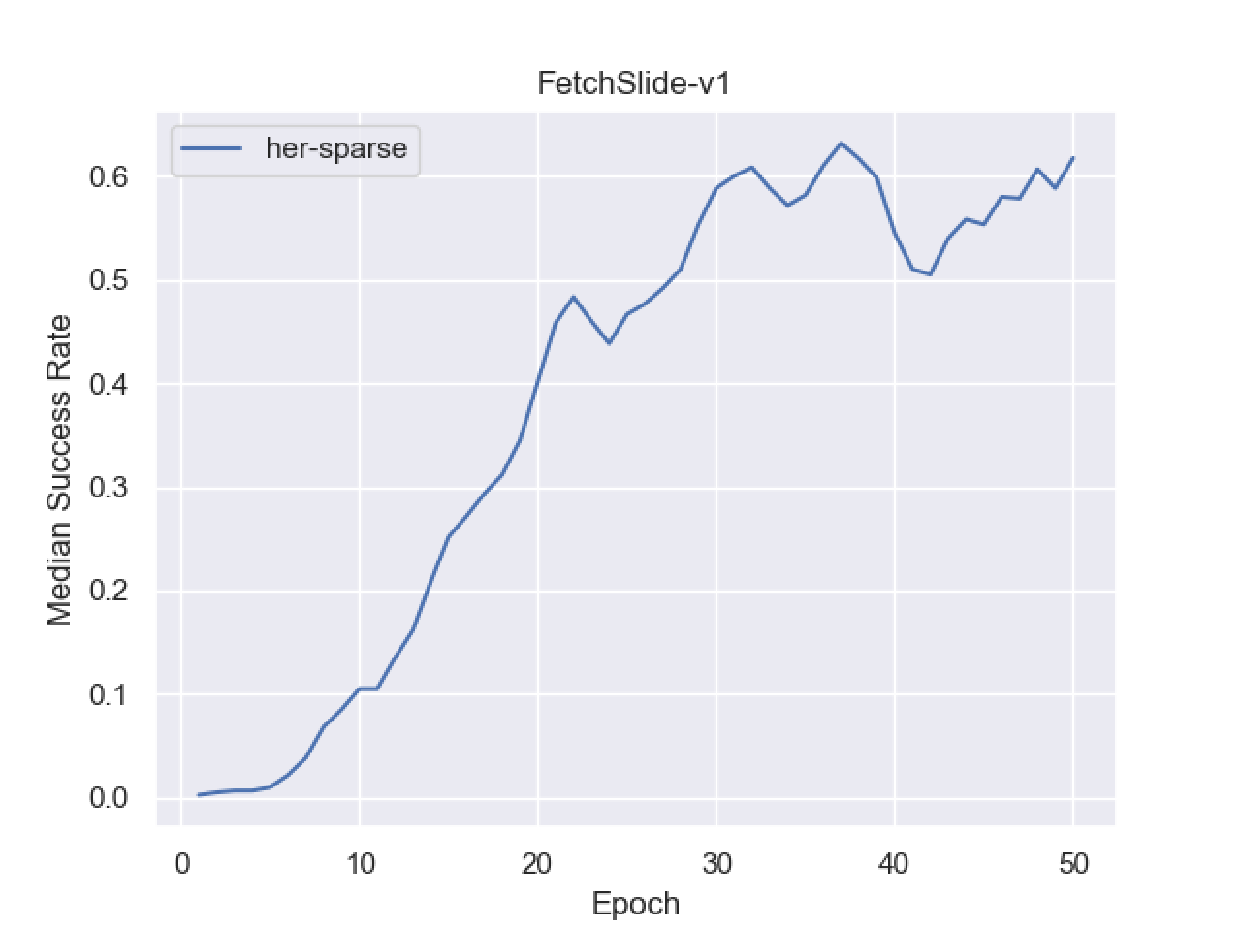
\includegraphics[width=0.49\textwidth]{figures/fig_FetchSlide-v1.pdf}\label{fig:fig_fetchslidea-v1}}
	\subfigure[FetchPickAndPlace-v1] {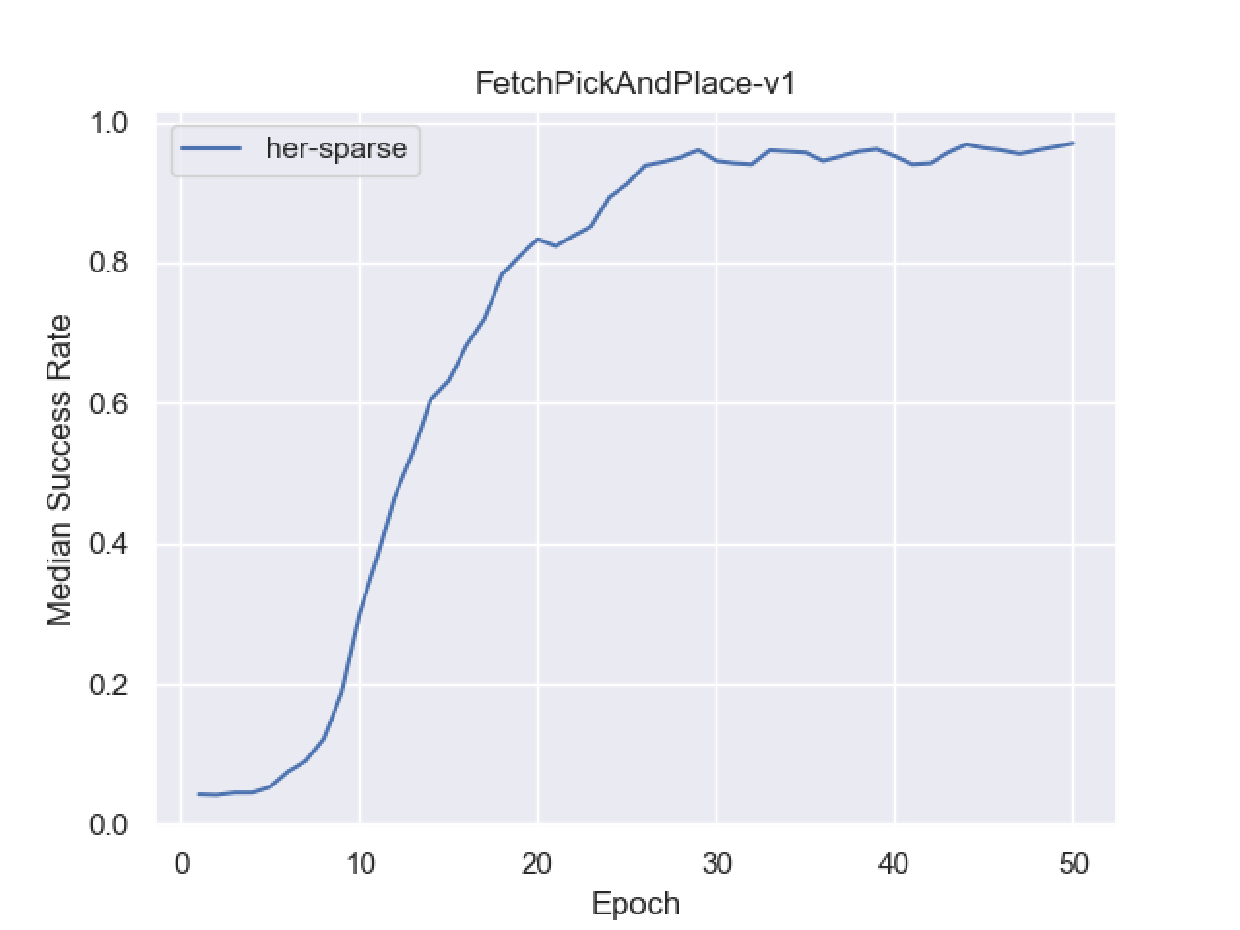
\includegraphics[width=0.49\textwidth]{figures/fig_FetchPickAndPlace-v1.pdf}\label{fig:fig_fetchpickandplace-v1a}}
	\caption{Success Rate of each task after 50 episodes of training}
	\label{benchm}
\end{figure}

Figure \ref{benchm} show the training results for each task.
FetchReach showed that just moving the robotic arm between two points is quite fast and easy to learn.
\newline
Obviously when comparing, the harder tasks FetchSlide and FetchPickAndPlace perform worse than FetchPush and FetchReach. FetchPickAndPlace in comparison to FetchPush introduced the difficulty of having to control opening and closing the gripper. Instead of having an action space with only 3 variables like for the other tasks, this action space is extended to 4 variables, which is an extension of the action space by 33\%. Having to learn how to grab the cube seems to take about 20 episodes longer than not needing to do it. 
%check exact number 
\newline
When comparing FetchSlide to FetchPush, the difference is clear. FetchSlide performs much worse. 
\newline
One difference between both tasks is the control over the object. In FetchSlide it is much harder to control the cylinder while moving it. The robot either has to hit it with very precise force or stop it if the goal position is in the robots' reach. Having big fluctuations between the force used and the distance the cylinder traveled makes it hard to learn how much force exactly is needed. 
\newline
Another difficulty is added by extending the range where the goal can be positioned. These multi-goal environments where the goal and object are in variable positions can be seen as a collection of many simple tasks, where each task is only about moving an object from a fixed position to another. Having a bigger goal space as increases the amount of these simple tasks greatly. As can be seen, these obstacles increase the difficulty drastically. 
%shortly summarize the obstacles ?




\section{FetchSlideball}

FetchSlideball is an extension to the environment FetchSlide. One of the future plans is to have an agent learn how to play golf. FetchSlideball made two differences to FetchSlide: the goal is put even farther in the distance and the cylinder was changed to a ball.
The task will be approached in smaller steps. 
%put this in extra section?
First a simple environment is tested where exactly the same environment as in FetchSlide is used and the only change is for the object to change from a cylinder to a ball. Through this test the difference in difficulty between using a cylinder and a ball is shown. This is needed to make FetchSlideball comparable to FetchSlide. 
Afterwards, for the following experiments, the friction and the steps per episode will be varied. 

\subsection{Task Description}

The task for FetchSlideball is exactly the same as for FetchSlide. The robotic arm has to push a ball from one position to another position, using the balls property to roll farther. Rolling the ball and sliding a cylinder might imply different friction types used, because a ball uses rolling friction instead of sliding friction which is usually much more lower. However, in this environment the same amount of friction is used for both objects. The main difference is the stability of the object. While the cylinder can fall on its side and slide different depending on where it is pushed, the ball stays stable. 
Also, other than in FetchSlide, the goal position is guaranteed to be outside the robots' reach. This should make it much harder for the agent to learn how to solve task.


\subsection{Environment}

\begin{figure} [!h]
	
	\centering
	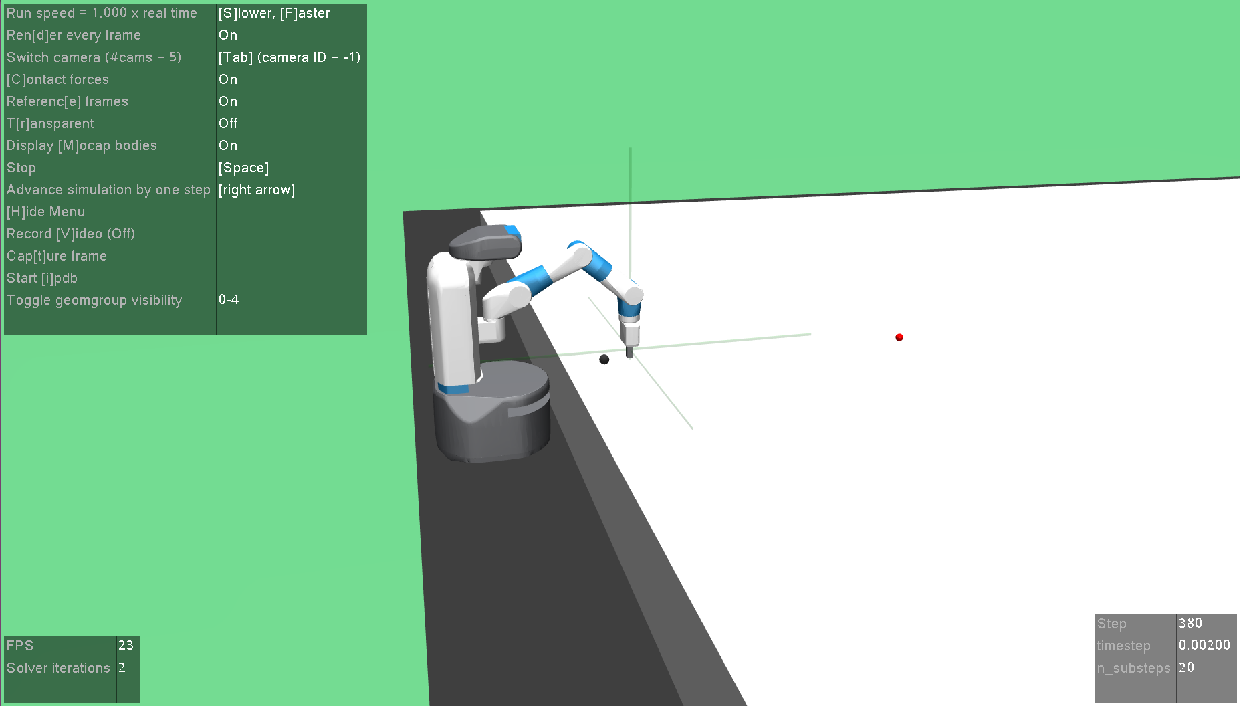
\includegraphics[width=1\textwidth]{figures/FetchSlideball-v3.pdf}
	\caption{FetchSlideball-v3}
	\label{slideball1}
\end{figure}

The environment can be seen in figure \ref{slideball1}. The size of the table was increased drastically. This was done to ensure that the goal would be on the table. The table is just much bigger than necessary to be able to accomodate future environments where the goal will be put in much farther distance. The object is a ball. As usual, there is a fetch robot and a red sphere marking the goal position. 

%put some experiment section for the differennt variables/versions used ?



\subsection{Results}


\begin{figure} [!h]
	
	\centering
	\subfigure[FetchSlide-v1] {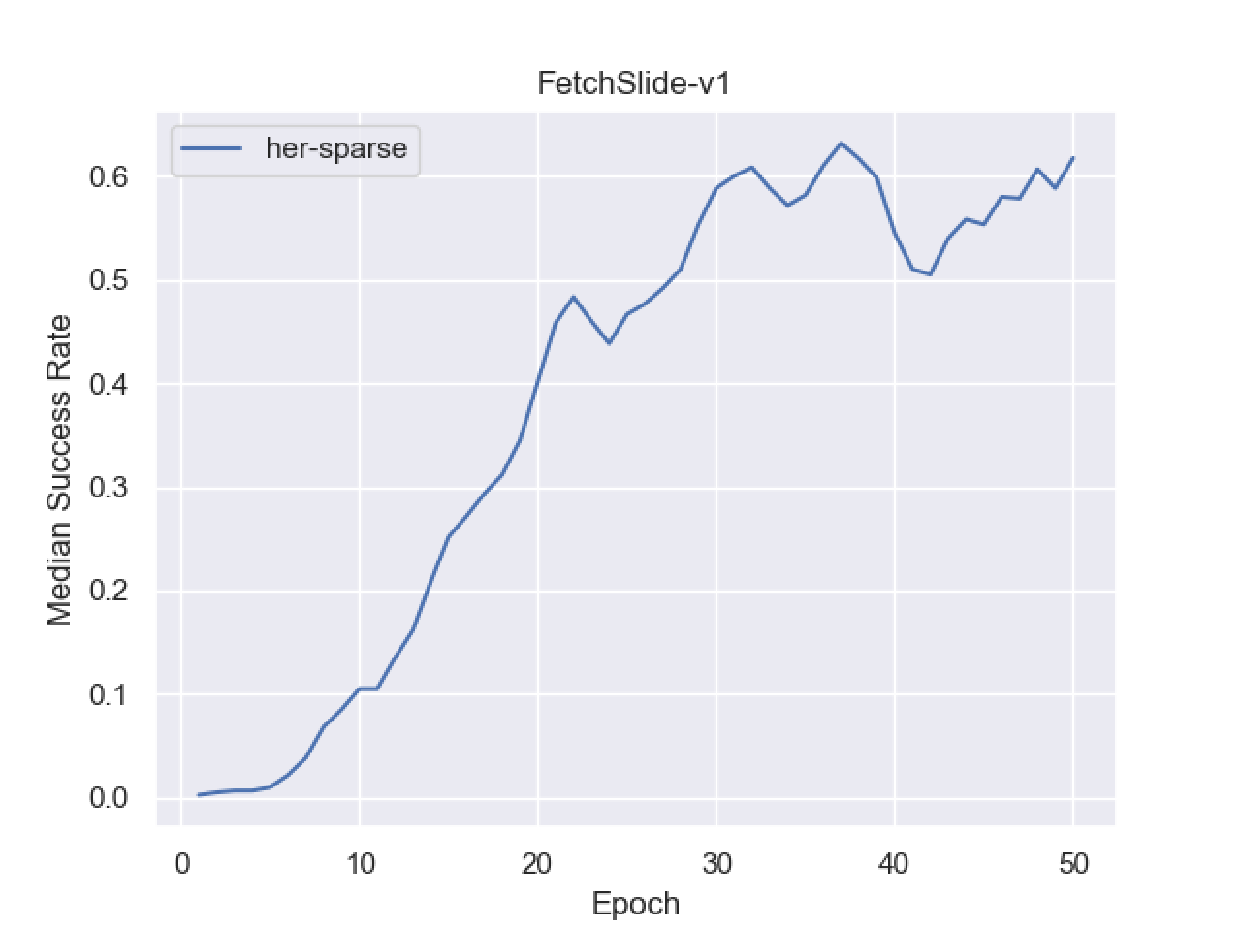
\includegraphics[width=0.49\textwidth]{figures/fig_FetchSlide-v1.pdf}\label{fig:fig_fetchslide-v1}}
	\subfigure[FetchSlideball-v1] {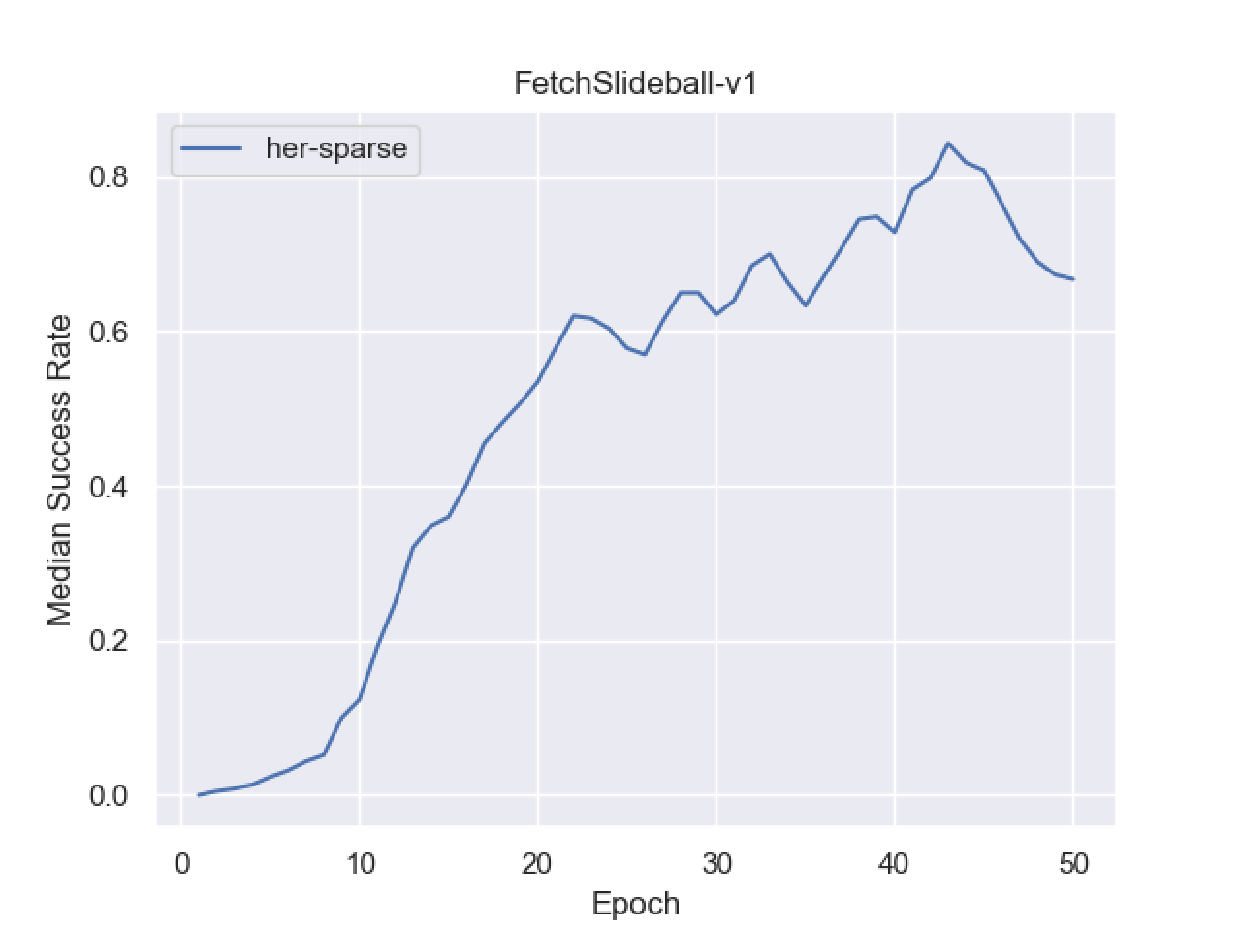
\includegraphics[width=0.49\textwidth]{figures/fig_FetchSlideball-v1.pdf}\label{fig:fig_fetchslideball-v1}}
	\caption{FetchSlide with a cylinder (left) and with a ball (right)}
	\label{slidecomp}
\end{figure}


First the FetchSlide environment was used with the only change being a ball. As can be seen in figure \ref{slidecomp}, FetchSlide with a ball performs much better than vanilla FetchSlide with a cylinder. Both learning curves are quite similar. They both have a success rate curve for the first 20 epochs. After the first 20 epochs, the success rate is still rising, but visibly slower. While FetchSlide with the cylinder only reaches a success rate of 60\%, FetchSlide with a ball reaches about 80\%. The difference might be explained by the ball being more stable. The cylinder that is used in the normal FetchSlide environment can fall over when it is moved at a bad angle, this can not happen to a ball.
%werid explanation, try to find out more
\newline
Afterwards the experiment continues for the FetchSlideball environment with a bigger distance. The new distance from start position of the ball to the goal position is about the doubled distance of the normal FetchSlide environment.
%fill in exact distances.
Training the FetchSlideball environment without changing any of the other parameters proved to be impossible as figure \ref{slideball2} shows. Later it was discovered to be because of a simple reason. The goal is too far away, so it is physically impossible for the robotic arm to roll the ball to the goal.
 
\begin{figure} [h]
	
	\centering
	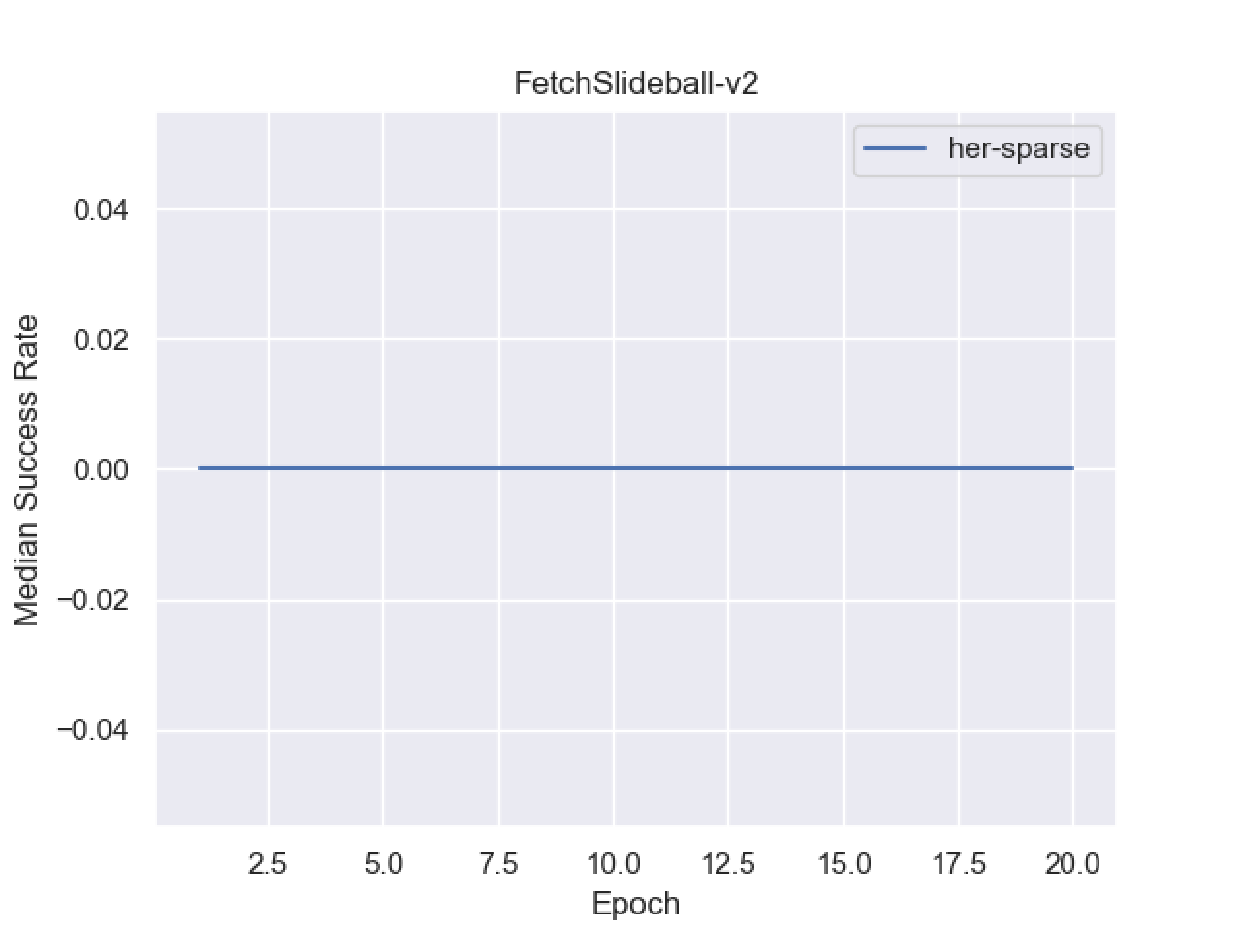
\includegraphics[width=1\textwidth]{figures/fig_FetchSlideball-v2.pdf}
	\caption{FetchSlideball with the same friction and timestep as in FetchSlide}
	\label{slideball2}
\end{figure}

Reducing the friction by 50\% made it barely possible to reach the goal. The goal could be reached, but the goal position is at the limit of the range that the ball could reach. Figure \ref{slideball3} showed how hard it is to learn to reach the goal. For the first 30 epochs, there was no success. Weirdly, at epochs 30 to 34 the goal was reached, but afterwards there was no success again. 
%some randomness ? but 4 episodes in a row ?
%TODO check this, maybe retry the experiment    

\begin{figure} [h]
	
	\centering
	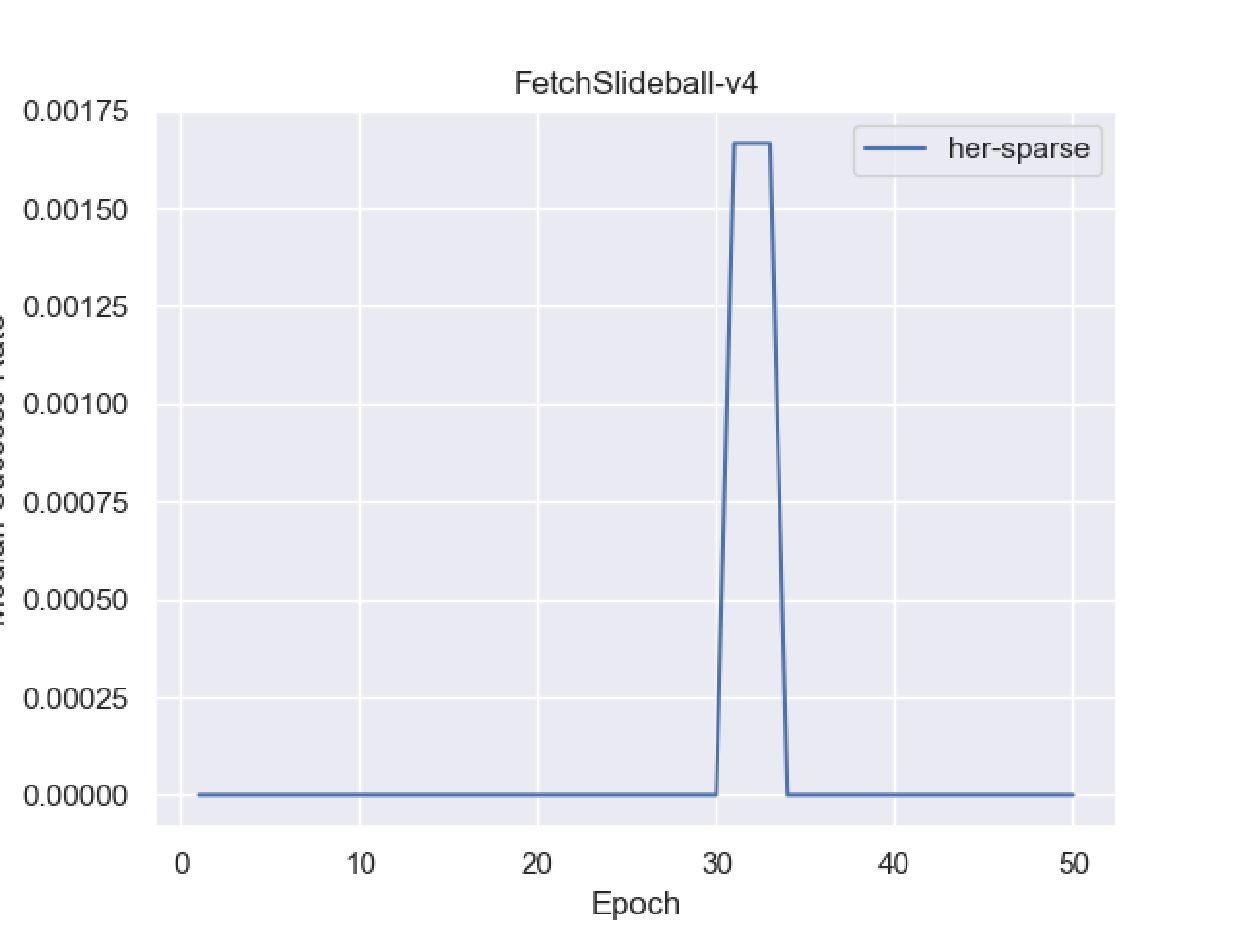
\includegraphics[width=1\textwidth]{figures/fig_FetchSlideball-v4.pdf}
	\caption{FetchSlideball with 50\% friction and more steps per episode}
	\label{slideball3}
\end{figure}

Changing the balls' friction to only 10\% of the original friction showed interesting results. As can be seen in figure \ref{slideball4}, for the first 15 epochs there is no success, but then the success rate slowly rose. At episode 47 the success rate spiked to almost the doubled success rate. The reason behind that shows how tricky the agent can be. Each training episode takes 1000 time steps. The episode is successful when the goal is reached, to be precise, in this environment if the ball is in a close range (0,05 units of length) of the goal position in the last time step.
The agent abuses this fact to solve the task different than intended. The intended solution is to roll the ball with just enough force, so that it stops at the exact goal position and stays there, so that the success condition is fulfilled and the task is successful solved. But the agent uses a different idea. It tries to hit the ball at exactly the right time, so that the ball is just at the goal position at time step 1000, the ball does not need to stop there. If the episode would take more time steps, then the ball would just roll too far, but because the episode ended at 1000 time steps, the success condition is fulfilled and the episode is counted as solved right.
But even in the cases where the episode is not successful, the robotic arm slides the ball in the right direction, it just rolls too far. When using the trained policy of the 10\% friction FetchSlideball environment to solve the task with 50\% friction, it is getting quite close to the goal because it learned to move the ball in the right direction.

%do 25% friction ?

\begin{figure} [h]
	
	\centering
	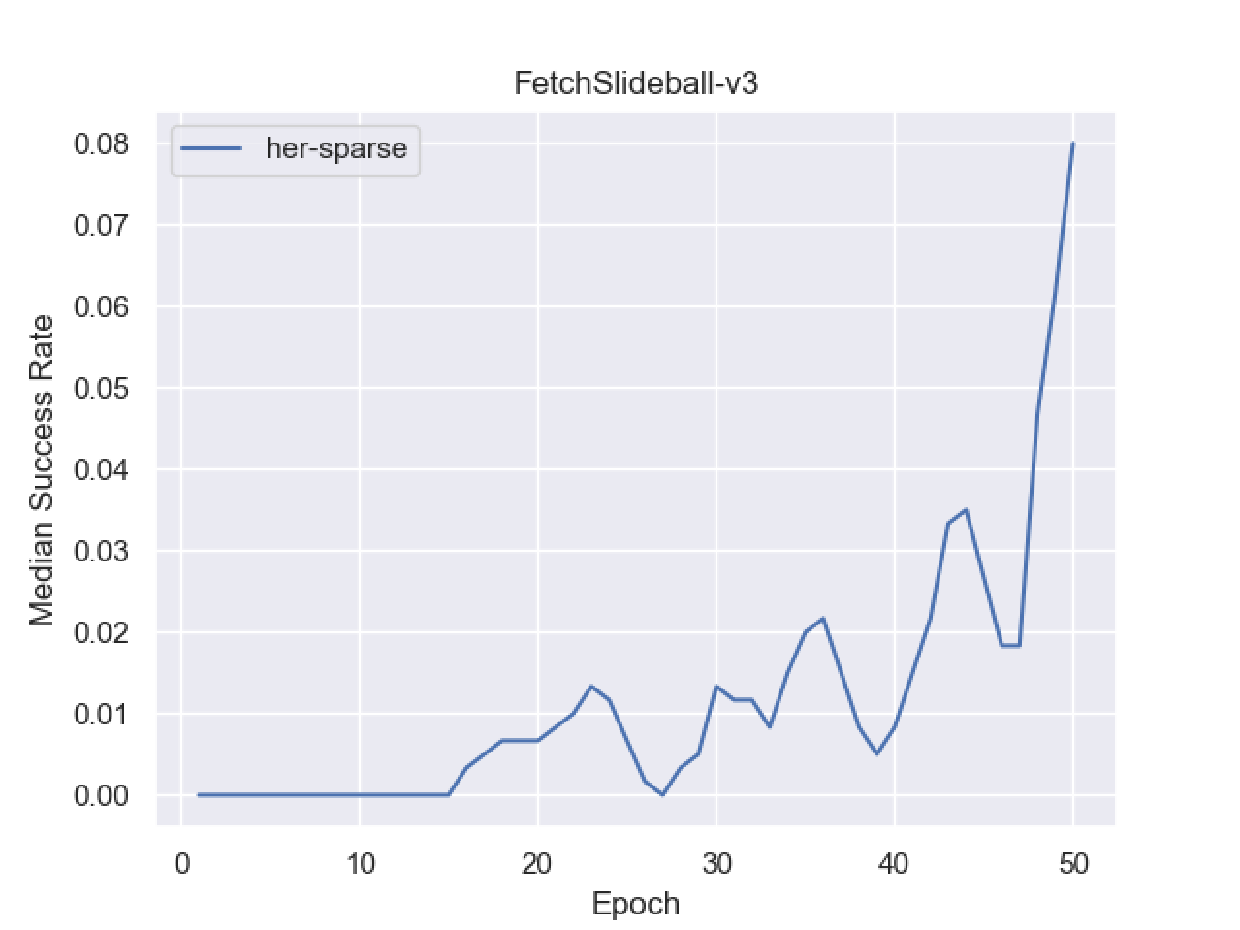
\includegraphics[width=1\textwidth]{figures/fig_FetchSlideball-v3.pdf}
	\caption{FetchSlideball with 10\% friction)}
	\label{slideball4}
\end{figure}

%do 10% friction, more time steps.

\subsection{Discussion}

Through these experiments two findings were learned. Using a ball instead of a cylinder improves the performance of the agent. This is attributed to the ball being a stable object. In this case, the ball showed an improvement of 33\% over the cylinder. It might be interesting to compare the ball to other objects. 
\newline
Also it was figured out that a bigger distance to the goal position increases the difficulty of the task greatly. For the FetchSlideball task with 10\% friction, only 8\% success rate could be reached after 50 episodes in comparison to the 60\% success rate by the FetchSlide task. And even for that 8\% success rate, the agent did not solve the task the intended way. 
\newline
This poses two questions: Is the difficulty solely rising due the fact that the goal distance is increasing or does the difficulty also depend on the proportion between goal distance and range where the robotic arm can roll the ball to? More experiments with different friction values have to be done to answer this question.
\newline
Also, how can the agent be prevented from solving the task in an unintended way ? To really solve the task in the intended way, the implementation of the task needs to be changed. The FetchSlideball task needs to change to have the ball lie on the goal position for some time, to count the task as successfully solved. This would prevent a ball that only touches the goal at the end to be counted.
\newline
The results have shown that vanilla HER can not solve these tasks where we increased the goal distance far outside the robotic arms' reach. To solve these tasks, further experiments with improved HER algorithms like Hindsight Goal Generation need to be done. As stated by Ren et al. \cite{hgg}, many hindsight experiences are not helpful to replay and therefore the hindsight goals need to be selected better to improve the performance. Especially in the case of the task FetchSlideball with 50 \% friction, the goal was located at the edge of the range where the robotic arm can roll the ball to. An approach where the agent is guided to roll the ball more often in the direction of the goal would improve the performance. Further research with improved HER approaches will be done in the future.

\section{FetchToss}

FetchToss is rather different than the other environments. For future plans, FetchToss is planned to become an environment that resembles basketball. The agent should learn how to throw a ball into a basket. This environment has similarities to FetchPickAndPlace and FetchSlide, because the gripper has to be used to grab a ball and the goal is also outside of the robotic arms' range. To solve the task, we first try to change the object to a ball and see how picking a ball compares to picking a cube.
Then a box is used to try to make the agent learn, how to toss the ball into the box.

\subsection{Task Description}

The task for FetchToss is to fetch a ball that is placed on the table and toss it into a box that is not reachable by the robotic arm without tossing. The goal has to be outside of reach to avoid having the robot just picking the ball up and putting it inside. The goal position and size is different than for the other tasks. For one, the goal this time is static, it will always be the same box at the same position. Also, the goal is much bigger this time. The task is fulfilled, when the ball is inside the box, it does not matter where in the box. The red sphere is just a visual mark, the actual goal is the whole box. The agent has to learn following steps: Pick up the ball like in FetchPickAndPlace, then move the object with enough force towards the goal and open the gripper to toss the ball and also hit the goal.


\subsection{Environment}

\begin{figure} [ht]
	
	\centering
	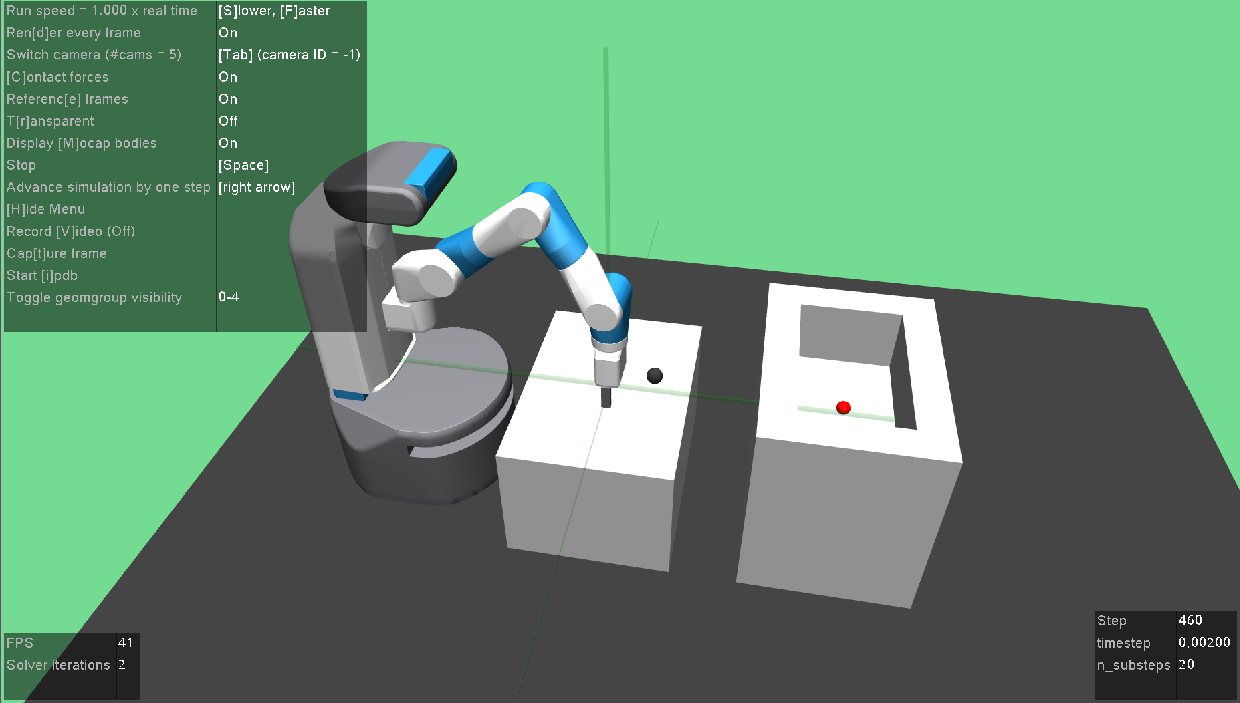
\includegraphics[width=1\textwidth]{figures/FetchToss-v1.pdf}
	\caption{FetchToss}
	\label{toss1}
\end{figure}

For this environment the environment of FetchPickAndPlace was used as a base. The object was also changed into a ball and a box was created to simulate as basket. As usual, there is also a fetch robot and a red sphere marking the goal. As mentioned, the actual goal contains the whole box, not only the position of the red sphere. Also, the goal is static.

\subsection{Results}

\begin{figure} [!ht]
	
	\centering
	\subfigure[FetchPickAndPlace-v1] {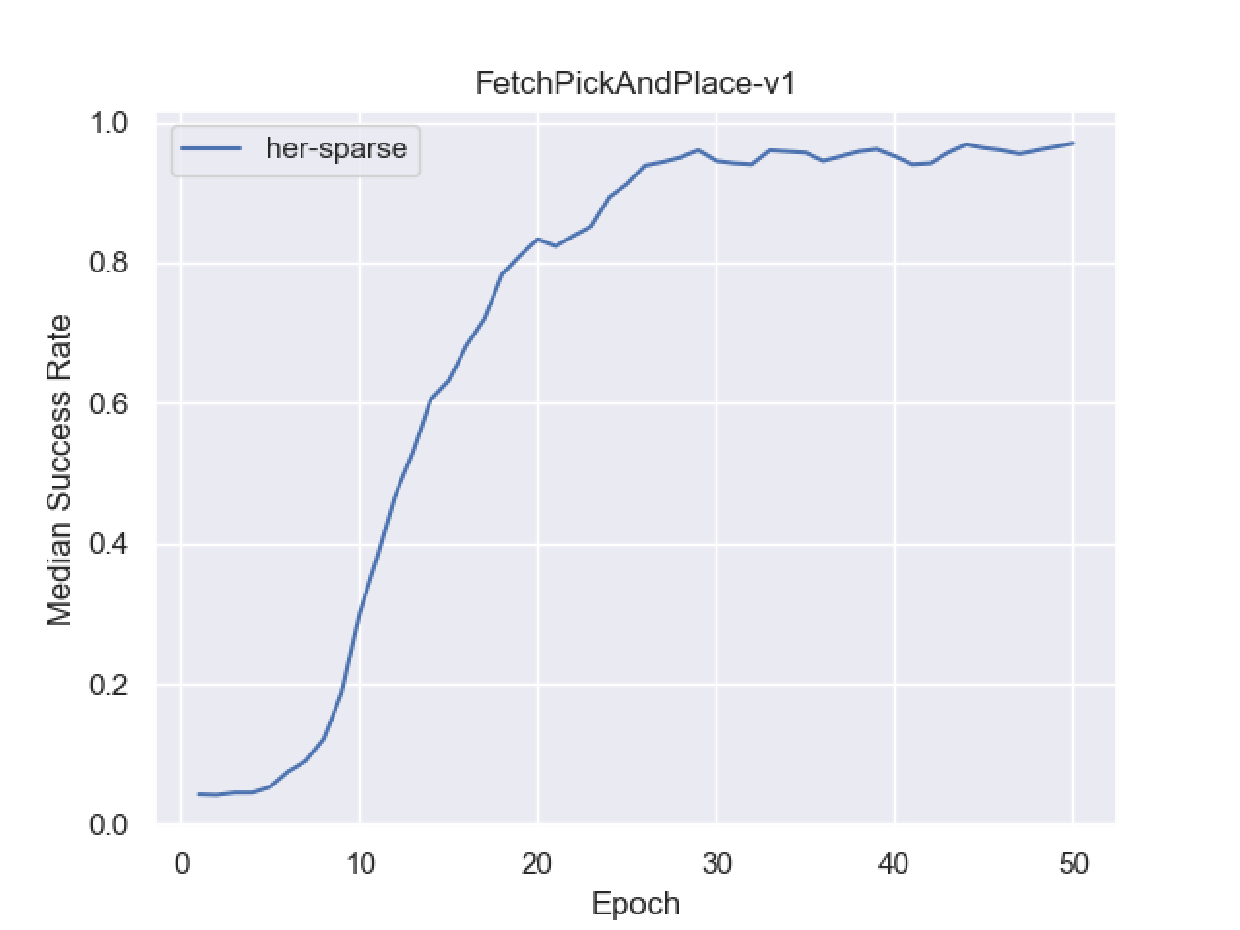
\includegraphics[width=0.49\textwidth]{figures/fig_FetchPickAndPlace-v1.pdf}\label{fig:fig_fetchpickandplace-v1}}
	\subfigure[FetchPickAndPlaceball-v1] {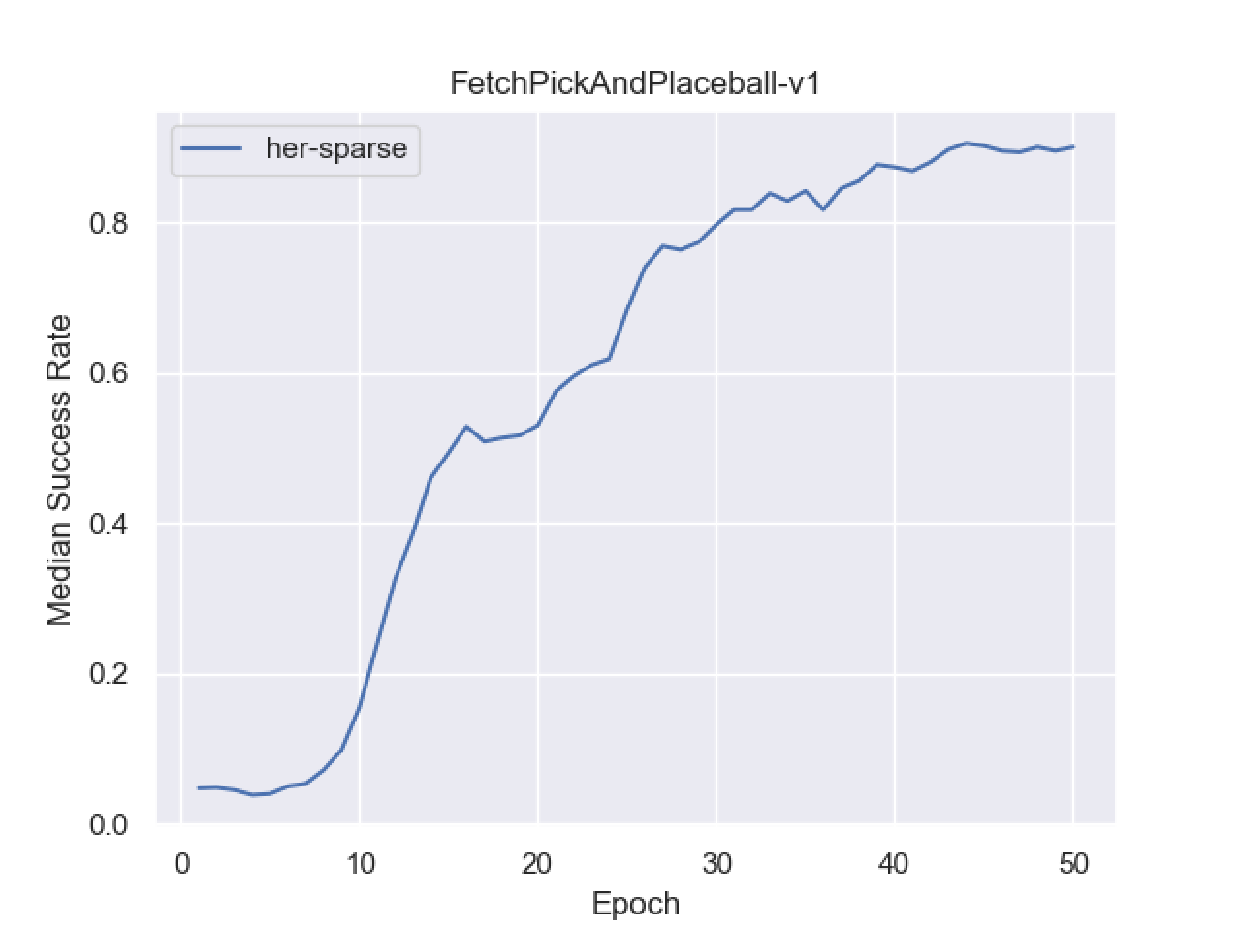
\includegraphics[width=0.49\textwidth]{figures/fig_FetchPickAndPlaceball-v1.pdf}\label{fig:fig_fetchpickandplaceball-v1}}
	\caption{FetchPickAndPlace with a cube(left) and a ball (right)}
	\label{pickballcube}
	
\end{figure}

As figure \ref{pickballcube} shows, picking up a ball instead of a cube seems to perform worse. Both show similar success rate curves. FetchPickAndPlaceball seems to differ at about epoch 15. While FetchPickAndPlace still has a steep success rate curve at epoch 15, FetchPichAndPlaceball already slows down with being more successful. Overall FetchPickAndPlace with the ball shows slightly lower success rates. While it reaches about 90\% success rate at 50 epochs, the vanilla FetchPickAndPlace with the cube reaches about 95\% success rate.

\begin{figure} [!ht]
	
	\centering
	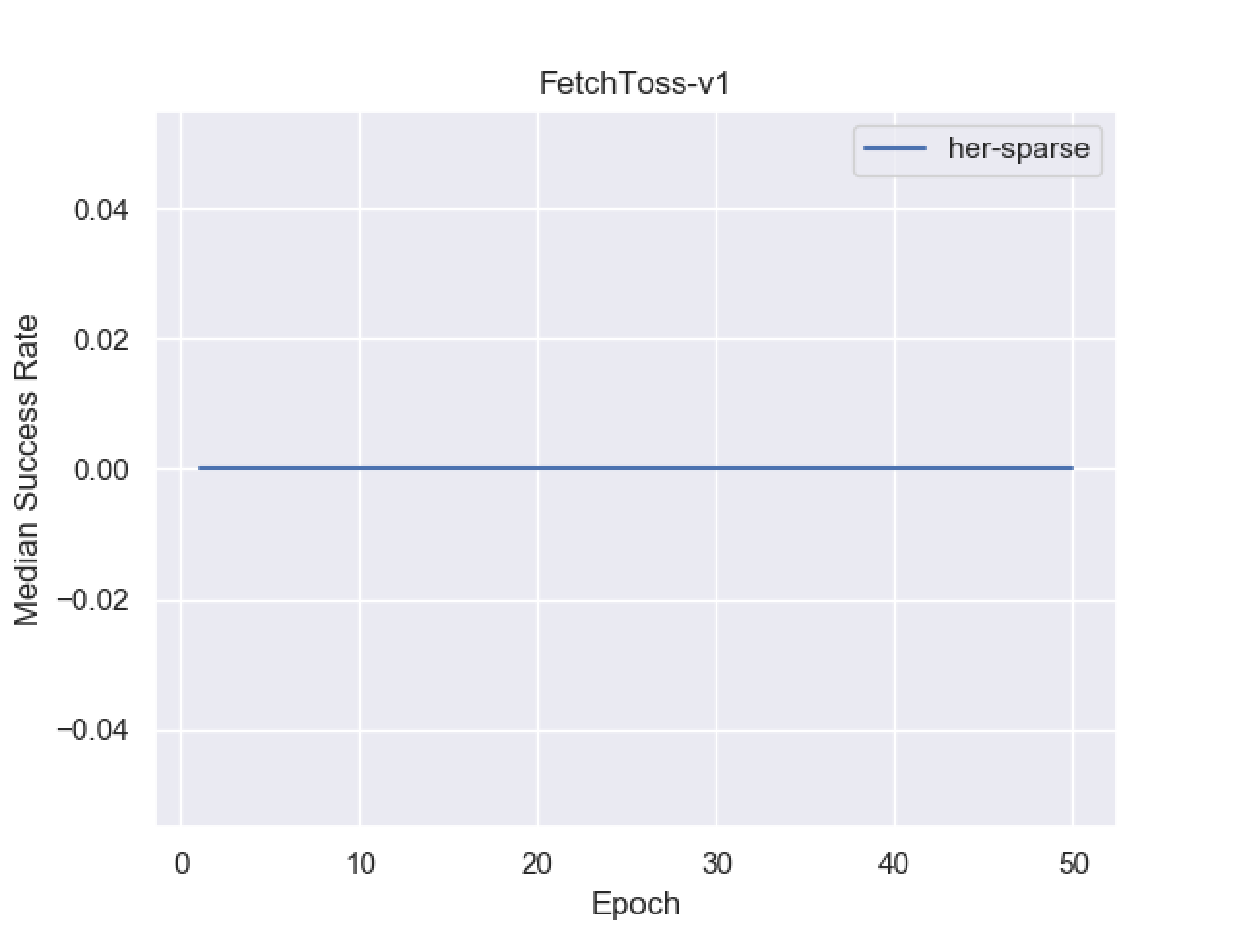
\includegraphics[width=1\textwidth]{figures/fig_FetchToss-v1.pdf}
	\caption{FetchToss}
	\label{toss2}
\end{figure}

Figure \ref{toss2} summarizes the results for the other experiments that were run. The robotic arm does not learn how to toss the ball at all. The box was changed to a box where the front is open to make it easier to toss in the back was made higher to prevent the agent from throwing the ball over the box. This also showed the same results. Another try was lengthening the time steps per episode from 1000 time steps to 2000 time steps, because it could just be impossible to solve the task as tossing takes some time. The ball was also made 100 times lighter (from 2 to 0.02 units of weight) which did not change the result. A path was planned manually to show if the reason for failing might be because the task itself is impossible. For the environment with the lighter ball a path to solve the task is possible which can be seen in Figure \ref{toss3}. This means that vanilla HER can not solve this task. Also tossing a cube instead of the ball does not work. This also proved to be unsuccessful. 

\begin{figure} [!h]
	
	\centering
	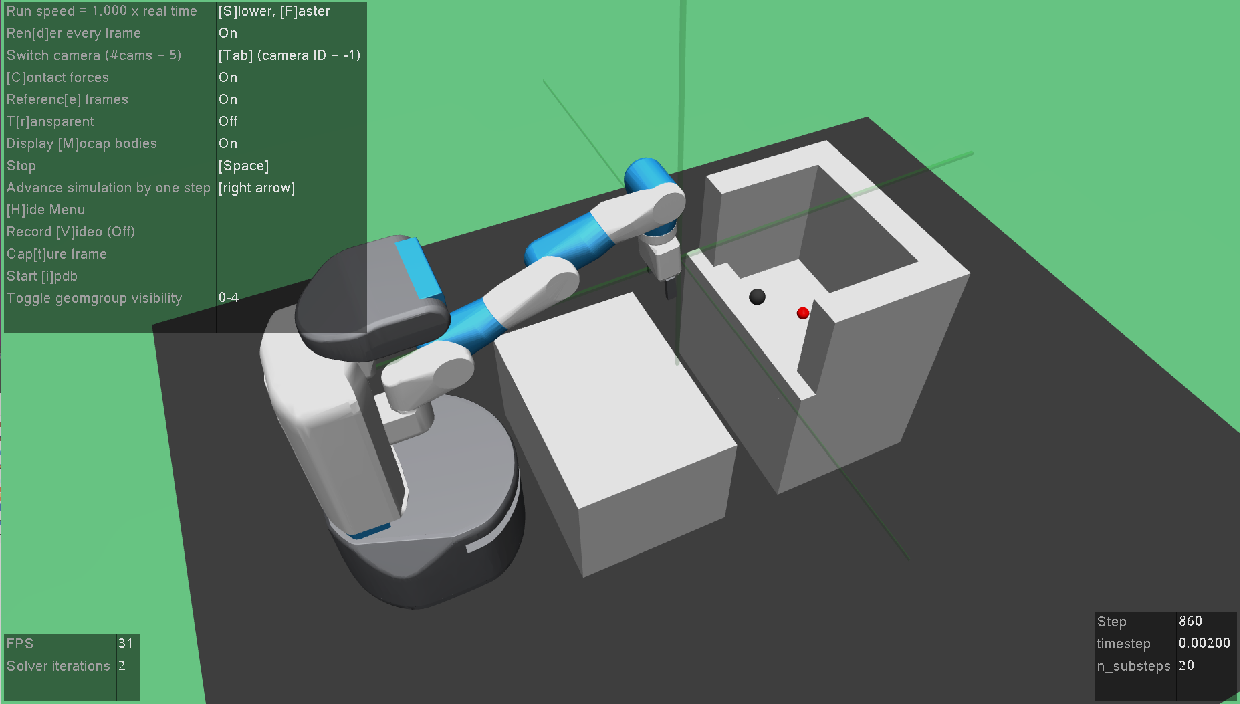
\includegraphics[width=1\textwidth]{figures/FetchToss-v0.pdf}
	\caption{FetchToss, with lighter ball and more time steps}
	\label{toss3}
\end{figure}

\subsection{Discussion}

Picking up a cube seemed to be easier than the ball. A reason might be because of their size form. A ball with radius of 0,02 units of length, and therefore a diameter of 0,04 units of length is simply smaller than a cube with each side being 0.04 units of length long. Even though both objects have 0,04 units of length at their longest part, the ball is just smaller. Also, because of the balls form, is has to be grabbed at the middle while the cube can be grabbed at any side, it will always be 0,04 units of length long. The cube is just easier to grab and harder to drop than a ball. Experiments could be done to figure out how big the ball has to show as much success as for the cube.
\newline 
Learning to toss the ball is pretty difficult as the results show. It was proven that the task is physically possible by finding a path for the lighter ball. So it seems that the task of tossing a ball is too hard to learn with standard HER.
\newline
As explained by Ren et al. \cite{hgg}, HER has the flaw that it learns how to solve goals that are equal to states that the agent already reached once, even though these goals might not be useful to learn how to solve the actual goal. In the FetchToss task learning how to toss the ball in the box seems to take too many difficult steps to learn. So vanilla HER fails. Improved HER algorithms might be useful to solve the task. Especially the energy-based hindsight experience prioritization approach by Zhao and Tresp \cite{energyher} might be useful for this task because tossing requires a lot of energy and therefore prioritizing replaying experiences with high energy would be especially fitting.
Further research in this direction will be done in the future.




		
		\chapter{Conclusion and Future Work}

Using RL for robotic arms has been difficult due to sparse rewards in robotic arm tasks. The concept of HER enabled working with sparse rewards by making the training samples more efficient through hindsight replay. Most of the research on HER focuses on improving the performance of HER. Instead in this thesis, harder tasks were constructed to use HER on. 
\newline
Two environments were built to test HER on, FetchSlideball and FetchToss. 
\newline
FetchSlideball is similar to the already existing task FetchSlide which is usually used as a benchmark for HER. The task involves using the robotic arm to slide an object to a point that might be outside of the robotic arms' reach. The only difference between both environments is that FetchSlideball uses a ball instead a cylinder and the distance to the goal was increased. We first tested the FetchSlide task with a ball and compared that to the cylinder used in the default FetchSlide task. The results showed that using a ball improved the success rate for this task by 20\% (from about 60\% to about 80\%). In a first experiment of the FetchSlideball task with the increased distance, the success rate was null. This was due to the ball not being able to roll far enough and therefore the task was impossible. To be able to reach the goal, the friction of the ball had to be modified. After halving the balls' friction the experiment was repeated. This time it was barely possible to reach the goal and solve the task, but the agent still showed almost no success. Reason for that is probably as Ren et al. stated \cite{hgg}, the goals that were learned through HER were not useful enough in learning how to solve the actual goal. Changing the balls friction to 10\% of its original friction showed interesting results. After 50 epochs, the success rate was at 8\%, which is an improvement to the former experiments. The agent learned to roll the ball in the right direction. However, instead of controlling the ball to stop at the right spot, the agent exploited the fact that a training episode only takes limited time and an episode is successful if the ball is in the goal space after the last time step. By rolling the ball with the right timing, the agent could get successful episodes by having the ball at the goal space when the episode ends - even though the ball would roll farther if the episode did not end. This showed that the agent at least learned how to roll the ball in the right direction, even for greater goal distances. 
\newline
FetchToss is a much harder environment. The agent is required to use the robotic arm to fetch a ball and toss it into a box that is slightly out of the robotic arms' range. First we compared fetching a ball in contrast to fetching a cube by comparing the FetchPickAndPlace task with a ball and cube. Fetching a ball proved to be about 5\% worse than fetching a cube (from about 95\% to about 90\%). When trying to train the agent to solve the FetchToss task, results showed no success at all. Even changing the box to make it easier to toss into, doubling the time steps for each episode, making the ball lighter or using a cube did not show any success. A path to solve the task was coded by hand which proved that it is possible to solve this task. It was just too hard for HER to solve. FetchToss requires many intermediate steps like finding the ball, picking it up, moving it in the right direction and releasing it with the right timing to toss it. Having all these steps increases the difficulty greatly. Using the energy-based experience prioritization approach by Zhao and Tresp \cite{energyher} in the future might help guide the agent to learn tossing because tossing requires a high amount of energy. 
\newline
This thesis showed that vanilla HER fails for both tasks FetchSlideball and FetchToss. For tasks with a high goal distance and very complicated solutions HER seemed to struggle.
Future work needs to focus on solving these tasks. An obvious approach would be to use improved HER algorithms like energy-based hindsight experience prioritization to solve these tasks. Also modifying these tasks might be a possibility for research. Finding out how much different goal distances affect the success rate might be interesting. After solutions are found to make these tasks work, these tasks could be extended to a golf and basketball environment as it was intended from the start. This could include using different obstacles like walls for a golf environment. Also, other objects could be used. It would be very interesting to research tossing paper planes.   
 
 
 
 
		
		% ---------------------------------------------------------------------------
		%
		% Appendix
		%
		% ---------------------------------------------------------------------------
		
		%\part*{Appendix}
		%\addcontentsline{toc}{part}{Appendix}
		
		\appendix %---------------------------------------
		
		\chapter{Simulation Parameters}

%\section{Detailed Validation Results}

\label{chapter:appendixA}

\begin{center}
	\begin{tabular}{| c | c |}
		\hline
		\_Q\_lr & 0.001 \\
		\_action\_l2 & 1.0 \\
		\_batch\_size & 256 \\
		\_buffer\_size & 1000000 \\
		\_clip\_obs & 200.0 \\
		\_hidden & 256 \\
		\_layers & 3 \\
		\_max\_u & 1.0 \\
		\_network\_class & baselines.her.actor\_critic:ActorCritic \\
		\_norm\_clip & 5 \\
		\_norm\_eps & 0.01 \\
		\_pi\_lr & 0.001 \\
		\_polyak & 0.95 \\
		\_relative\_goals & False \\
		\_scope & ddpg \\
		aux\_loss\_weight & 0.0078 \\
		bc\_loss & 0 \\
		demo\_batch\_size & 128 \\
		gamma & 0.98 \\
		n\_batches & 40 \\
		n\_test\_rollouts & 10 \\
		noise\_eps & 0.2 \\
		num\_demo & 100 \\
		prm\_loss\_weight & 0.001 \\
		q\_filter & 0 \\
		random\_eps & 0.3 \\
		replay\_k & 4 \\
		replay\_strategy & future \\
		rollout\_batch\_size & 2 \\
		test\_with\_polyak & False \\
		\hline
	\end{tabular}
\end{center}




		%\chapter{Setup Instructions}

\label{chapter:appendixB}

%TODO DELETE

This section provides an overview of the procedures needed to run the benchmarks from the source code package included for this thesis.
The Ubuntu 14.04 OS is assumed.


The following commands install the Altera ICD on the system:
\begin{lstlisting}[label={}, caption={}]
sudo mkdir /etc/OpenCL/AlteraICD
sudo cp -r altera_icd/bin/* /etc/OpenCL/AlteraICD
sudo sh -c "echo '/etc/OpenCL/AlteraICD/libalteraicd.so.1' \
     >> /etc/OpenCL/vendors/altera.icd"
\end{lstlisting}

The modified Altera PCIe module can be compiled with the following script:
\begin{lstlisting}[label={}, caption={}]
./make_all.sh
\end{lstlisting}

The modified NVIDIA module can be compiled with the following command:
\begin{lstlisting}[label={}, caption={}]
make module
\end{lstlisting}

To load the modified modules, the original modules have to be removed first.
Since the display manager depends on the NVIDIA module it must be stopped too.
To do this, the TTY has to be switched, e.g. with the key combination \texttt{CTRL+ALT+F4}.
Then, the following command sequence will replace the modules:
\begin{lstlisting}[label={}, caption={}]
sudo service lightdm stop
sudo rmmod nvidia-uvm aclpci_drv nvidia
sudo insmod nvidia.ko
sudo insmod aclpci_drv.ko
sudo service lightdm start
\end{lstlisting}

To load the modules automatically during the boot procedure, the previous modules should be overwritten:
\begin{lstlisting}[label={}, caption={}]
sudo cp aclpci_drv.ko /lib/modules/$(uname -r)/misc/
sudo cp nvidia.ko /lib/modules/$(uname -r)/kernel/drivers/
\end{lstlisting}

For testing, the code from appendix \ref{chapter:appendixA} or the provided benchmark \texttt{direct\_benchmark} can be used.



		
	


  \clearemptydoublepage
 

     \listoffigures{}


	\bibliography{bibliography/literature}
	

\end{document}

